\documentclass[a4paper,12pt]{report}
\usepackage[center]{caption}
\usepackage[pdftex]{graphicx}
\usepackage[pdftex]{hyperref}
\usepackage{amsmath}
\usepackage{subfig}
\usepackage{listings}

% From wikipedia
\DeclareMathOperator*{\argmax}{arg\,max}
\DeclareMathOperator*{\argmin}{arg\,min}

\lstset{breaklines=true,basicstyle=\small,tabsize=3,numbers=left,numberstyle=\tiny,numbersep=5pt,emptylines=1}

\lstdefinelanguage{Cg}
	{morekeywords={const,float,float2,float3,float4,float4x4,uniform,in,out,sampler3D,int,void,TEXCOORD0,COLOR0,TEXUNIT0,TEXUNIT1,cos,sin,return,for},
	sensitive=true,
	morecomment=[l]{//},
	}

\title{An Investigation into the Generation of 3D Skeletal Models from Voxel Data and their use in Gait Recognition}
\author{David Sansome}

\begin{document}
\bibliographystyle{plain}

\maketitle

\begin{abstract}
	This report describes the progress made into developing a 3D model-fitting application.
	The techniques of filter correlation and active contours are explored in detail, and their use in fitting a model to a reconstructed 3D image is examined.
	Stream-processor implementations are considered as a means of improving the performance of the algorithms.
	Preliminary results have been obtained from these methods, but there is much room for improvement.
	An extension to the filter correlation method is proposed that aims to resolve some of the problems observed during development.
\end{abstract}

\newpage

\tableofcontents

\chapter{Introduction and background}

\section{Overview}

\begin{figure}[b]
	\centering
	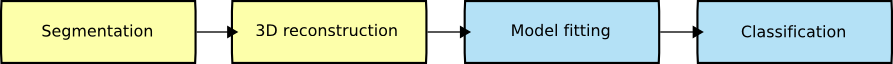
\includegraphics[width=12cm]{overview.png}
	\caption{The main stages in gait recognition.
		Those coloured blue are the ones tackled in this project.}
	\label{OverviewBoxes}
\end{figure}

What is gait recognition.
Input data.
Data from Southampton Gait Tunnel.
Number of cameras.


\clearpage
\section{Project goals}

\subsection{Model fitting}

The primary goal of the project is to produce an application that can process voxel data of a walking figure and generate a simple 3D skeletal model.
In its simplest form the model will consist of four cylinders representing the thighs and lower legs.
The angles these cylinders make with each other and the hips will be measured and stored to be used as part of the figure's identifying information.

The application should also able to track the movement of the parts of the model over subsequent frames of a video.
It should take advantage of the temporal continuity of human gait - that the change in position of a certain point on a person's torso between frames is quite small.
This can be used to simplify model-fitting across multiple frames -
the position of the model in the last frame can be used as a starting point and can narrow down the possible model positions of subsequent frames.


\subsection{Real-time}

One of the most interesting aspects of gait-recognition is its applicability to security, and the advantages of being able to identify people from a distance without their knowledge.
For gait systems to be of use in real-world environments they should make use of efficient image-analysis techniques and be able to identify people quickly.
A system should be able to raise an alert as soon as possible after a target figure moves into the surveillance area, and not be dependent on slow image-processing implementations.

While it might not be possible to make this process truly real-time, it is one of the goals of this project to investigate ways to improve the performance of gait and its ability to produce results more quickly.


\subsection{Gait recognition}

The eventual goal of this work on model-fitting is to be able to identify and recognise the gait of figures captured in video.
Analysis will need to be performed to determine how useful the data derived from the models is to gait recognition.
This analysis will primarily take the form of investigations into existing research on gait recognition, specifically into the type of data required from image segmentation such as dimensions and angles.


\subsection{Additional work}

As an additional task if time permits, research will be done into the possibility of covering additional parts of the body in the model fitting process.
The basic model consists of thighs and lower legs.
More useful information may be gleaned by analysing the motion of other limbs such as the arms.
Rotation of the torso may also be considered.
\clearpage
\section{Previous work and supporting literature}

This project builds heavily on previous research and development work by members of the University of Southampton.
The sample data used was obtained from test subjects walking through the Southampton Gait Tunnel.
Their movements were recorded on a number of cameras and the images processed by various segmentation and 3D reconstruction algorithms.

The remainder of this section covers the additional work that has been useful in the development of the project.

\subsection{Model-fitting}

In \cite{GaitBook} Nixon et al.\ summarise the general approach to model-based gait recognition.
The important angles between the limbs for consideration are shown to be those along the direction of movement.
A Pose Evaluation Function (PEF) is described that can be used to improve and measure the error of a particular fitting of a model to an image.
Both boundary and region matching errors are considered when calculating this function, reducing the chance that a model segment will be placed in the empty space between two limbs.

\bigskip
\noindent In \cite{cardboardpeople} Michael et al.\ describe an approach to model fitting entitled ``Cardboard People''.
Limbs in the model are represented by rigid planar patches.
These are connected together in a chain structure, with each rectangular plane consisting of four articulated points.
While the research presents an interesting approach to model-fitting, the technique is strictly 2D and therefore not directly applicable to this project.

\bigskip
\noindent Zhihui et al.\ \cite{LinearModelFitting} describe a human body model and show how linear regression can be used to fit it to an image.
The method of least squares is used in the paper to align points on the model to their corresponding locations on the human body shown the image.
This method shows some very promising results, with the two main problems listed in the paper being caused by inaccurate or noisy segmentation.
There is less of an issue in the Southampton sample data which is relatively free of noise.

\subsection{Active contours}\label{ContourBackground}

In \cite{CohenBalloons}, Cohen presents a model for active contours that considers the curve as a ``balloon'' that is inflated by a balloon force.
This force takes the form:

\begin{equation}
	F = k_1 \vec{n}(s) - k\frac{\nabla P}{\|\nabla P\|}
\end{equation}

\noindent Where $\vec{n}(s)$ is the normal vector to the curve and $P$ is the image force.
This force makes our contour expand like a balloon to fill a space, stopping when it encounters an opposing force from features of the image.

\bigskip
\noindent Gunn and Nixon present another force in \cite{GunnSnake} that causes an active contour to take the shape of a circle.
This force $\mathbf{e}_i$ on the snaxel $i$ at position $\mathbf{V}_i$ is calculated from the neighbouring snaxels by:

\begin{equation}
	\mathbf{e}_i = \tfrac{1}{2}(\mathbf{V}_{i-1} + \mathbf{V}_{i+1}) - \mathbf{V}_i + \theta_i\tfrac{1}{2}\mathbf{R}(\mathbf{V}_{i-1} - \mathbf{V}_{i+1})
\end{equation}

\noindent Where $\mathbf{R}$ is a $+90^\circ$ rotation matrix.
$\theta$ is the angle that should exist between a snaxel and its neighbours in order for them to form a circular shape.
This angle is defined by $\theta = tan(\frac{\pi}{N})$ where $N$ is the number of snaxels.

\bigskip
\noindent Williams and Shah \cite{SnakeAlgorithm} present a fast algorithm for implementing active contours.
A dynamic programming approach is used to avoid having to conduct an exhaustive search of the entire image.
During each iteration the neighbourhood of each snaxel is examined, and the point in the neighbourhood that gives the smallest energy is chosen as the new location for the snaxel.
Iteration continues until the number of points moved falls below a threshold.

\bigskip
\noindent In \cite{ImageSegModels} Xu et al.\ present a novel approach to image segmentation.
Active Shape Models, originally proposed by Cootes et al.\ in \cite{cootes93use} and \cite{cootes95}, define a set of points that represent a particular feature in the image.
During training these points are manually drawn on each image in the set of training data.
The eigenvectors are then extracted from the training set and principle components analysis (PCA) used to select those that are most important.

The model can be fitted to new images by both applying transformations to it (translation, rotation and scale) and by adjusting the weights of the eigenvectors (referred to as the \emph{shape parameters}).
This is performed iteratively and stops when changes in the pose and shape parameters are insignificant.

While interesting, this approach seems very generic and more suited to matching complex shapes.
For matching a simple cylinder representing a thigh, the algorithm may be considered overkill.

\subsection{Gait recognition}

Research into gait recognition has typically been split into two areas - model-based analysis and model-free analysis.
Model-free approaches use some form of statistical or spatiotemporal analysis on a sequence of frames - typically after segmentation and background subtraction.
Model-based approaches first seek to develop a model for the motion of limbs, and then describe the subject using the values of the parameters for that model.

One of the earliest works in model-free analysis was produced in 2004 by Niyogi and Adelson \cite{XYT}.
They used the spatiotemporal patterns of the head and legs both for gait detection (determining whether there is a person walking in the field of view) and gait recognition (determining \emph{who} that person is).
In \cite{EigenRecognition} Murase and Sakai present a method using Principal Components Analysis (PCA) and correlation in a parametric eigenspace representation.
Shutler and Nixon \cite{ZernikeMoments} use statistical moments to gather information from velocity as well as shape.

\bigskip
\noindent Model-based approaches have a number of advantages over statistical methods.
Wagg and Nixon describe some of these advantages in \cite{ecs9374}:
``Using a model ensures that only image data corresponding to allowable human shape and motion is extracted, reducing the effects of noise.
This also means that gait dynamics are extracted directly by determining joint positions, rather than inferring dynamics
from other measures.''

\bigskip
\noindent Cunado et al.\ present a detailed background to the various gait recognition approaches in \cite{GaitModels}.
The paper describes which of the limbs provide the most useful information for gait.
The smaller and easily obscured body parts such as the ankle and pelvis tend to provide useful identifying information, however identifying these from noisy images can be very difficult.

The focus of the paper is on the angle made by the thigh with the hip, the thigh and calf being modelled as simple pendulae.

\bigskip
\noindent In his PHD thesis \cite{KarlSharman} Sharman lists 23 parameters that are required for simple gait recognition.
Among these are the central position of the hip at time $t = 0$, the thigh length, and the harmonics of oscillations of hip positions both vertically and in the direction of travel.


\subsection{GPU processing}

Today's CPUs are very good at performing serial programming tasks.
However as Owens explains in \cite{GemsStreams} this serial programming model is poorly suited to many high-performance applications that process large amounts of data.
Typically these applications will perform the same operations on a large body of similar data (such as pixels).

A better programming model for these applications is that of the stream processor.
Stream processors (such as those found in modern graphics cards) run a computational \emph{kernel} over a stream of either simple (floating point valued) or complex (structured or vector) data.
In normal 3D graphics applications these streams are typically made up of geometry data such as triangles, and the kernels are the fixed-function lighting and shading programs.
However in recent years graphics cards have evolved to allow arbitrary kernels to be executed on custom user-specified data streams.
Using languages such as Cg \cite{CgToolkit} and CUDA \cite{CudaToolkit}, the application developer can completely customise the operation of the stream processor.

\bigskip
\noindent In \cite{GemsVision} Fung demonstrates how typical computer vision algorithms can be implemented on the GPU.
Canny edge detectors, a motion tracking algorithm and a Gaussian blur are implemented in the Cg programming language.

\chapter{Design approaches}

\section{Modelfitting framework}

In the early stages of the project it was decided that it would be necessary to create a custom application to process and display voxel data.
The rationale behind doing this instead of using an existing solution such as Matlab or Octave was threefold:

\begin{enumerate}
	\item The sample dataset from the Southampton Gait Tunnel is stored in a custom binary format, the parsing and display of which is
		undertaken by an C library, Vis4D, written by Richard Seely.
		The library is efficient and well-tested, therefore it would be beneficial to make as much use of it as possible.
	\item One of the goals of the project is to investigate ways in which the algorithms can be made parallelizable and applicable to real-time processing.
		As a prototyping language Matlab is generally less suitable for real-time or high-performance computing than a lower-level language such as C.
	\item The key aspect of this area of research that sets it aside from others in the field is that it focuses on 3D datasets.
		Visualising this 3D data in a useful way will require a custom user interface.
\end{enumerate}

It was decided to create an application that would load and process sequences of frames containing voxel data.
The application would run image-processing and classification algorithms on the data, and would be capable of handling both
the conventional and stream-processor implementations that are described throughout this chapter.

%The algorithms would be implemented as pixel-shaders, using the stream-processor capabilities of the GPU to execute code on hundreds of pixels at once.

Qt \cite{Qt} was chosen as the user-interface toolkit due to its excellent API and developer documentation.
Another advantage of using Qt is for its cross-platform compatibility - applications written using the toolkit can be compiled
for Linux, Mac OS X and Windows with no changes to the source code.
OpenGL along with the NVIDIA Cg Toolkit \cite{CgToolkit} provide a solid cross-platform foundation on which to build the shader components.

\begin{figure}[tb]
	\centering
	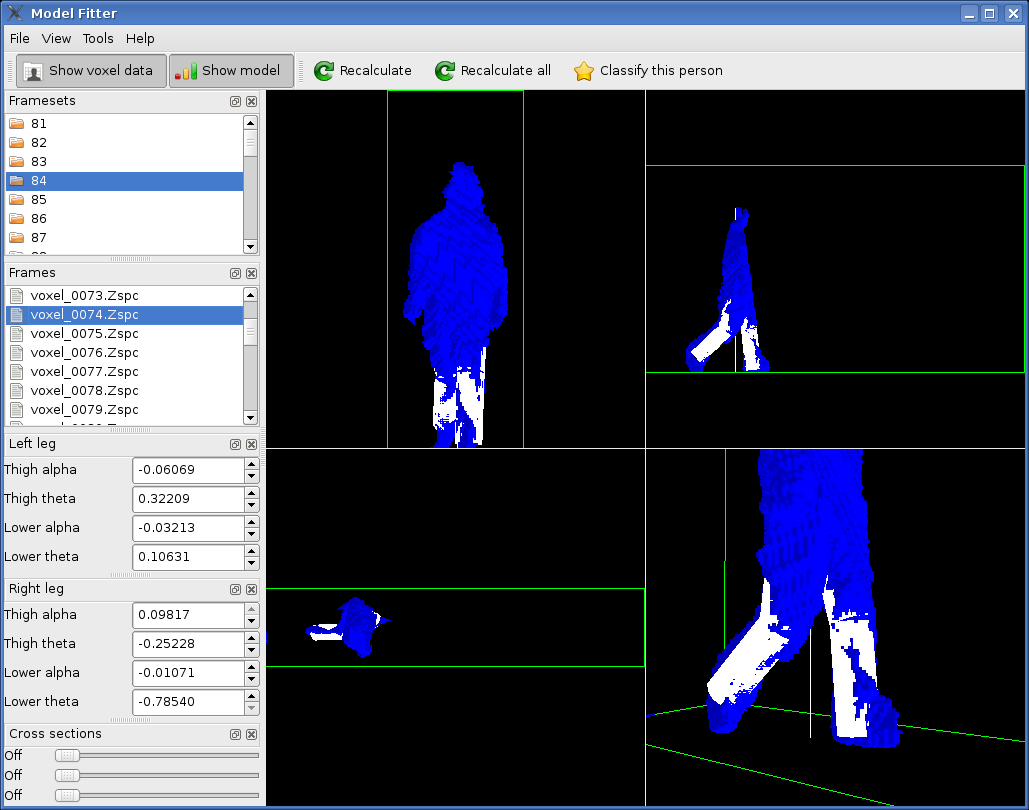
\includegraphics[height=8cm]{screenshot.png}
	\caption{Screenshot of the ``Model Fitter'' application.}
	\label{Screenshot}
\end{figure}

Figure \ref{Screenshot} shows a screenshot of the application in its completed state running under X11 on Linux.

\bigskip
The remainder of this chapter will describe the various algorithms implemented in the Model Fitter application,
and explain which of them were successful.\clearpage
\section{Pre-processing}\label{LocatingCenter}

A number of pre-processing steps are required before running any kind of modelfitting process on a frame.
Several pieces of information are gathered:

\begin{enumerate}
	\item The greatest z value for a filled voxel.
		This is used to determine the height of the figure.
		Half this height is assumed to be the height of the hips.
	\item The mean coordinate.
		This is taken to represent the centre of the figure and is used to normalise his position as he walks across the frame.
		It is calculated as follows:
		\begin{equation}
			\mathbf{V}_{mean} = (\overline{x}, \overline{y})
		\end{equation}
		Where
		\begin{align}
			\overline{x} &= \frac{1}{s_x s_y s_z} \sum_{x=1}^{s_x} \sum_{y=1}^{s_y} \sum_{z=1}^{s_z} x I(x,y,z) \\
			\overline{y} &= \frac{1}{s_x s_y s_z} \sum_{x=1}^{s_x} \sum_{y=1}^{s_y} \sum_{z=1}^{s_z} y I(x,y,z)
		\end{align}
	\item The width, or x-extent, of the subject.
		This is calculated simply by finding the largest and the smallest x coordinate.
\end{enumerate}

The key assumption made here is that a subject's legs ``start'' half way between his feet and the top of his head.
Figure \ref{Preprocessing} demonstrates this by showing how the greatest z value for a filled voxel, $h$, is used to
indicate the starting position of the legs.

\begin{figure}[b]
	\centering
	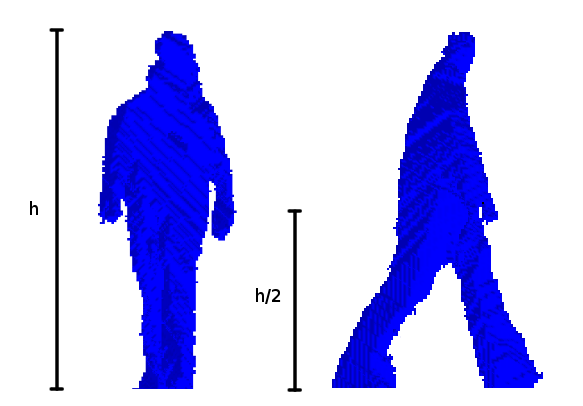
\includegraphics[height=6cm]{preprocessing.png}
	\caption{The information gathered during the pre-processing step is used as a guide for where to start searching for the legs.}
	\label{Preprocessing}
\end{figure}
\clearpage
\section{A model for human gait}
\label{Design:Model}

Before discussing any details of the algorithms used, it may be helpful to define exactly which parameters
we are trying to extract from each frame of the animation.

Figure \ref{ModelImages} shows our model for the human leg.
At the top of the model is the hip which, as we saw earlier, is fixed half-way between the ground and the subject's head.
Connected to this is the thigh which is free to pivot about the hip in two axes.
The angles the thigh makes with the vertical are denoted by $\theta$ and $\alpha$.
$\theta$ is the angle in the direction of travel, and $\alpha$ is the angle perpendicular to the direction of travel.

As we shall discover later, $\theta$ has a very large range of $\pm \frac{\pi}{4}$.
$\alpha$ is more restricted, typically falling between $\pm \frac{\pi}{32}$.

\begin{figure}[hb]
	\centering
	\subfloat[Side view]{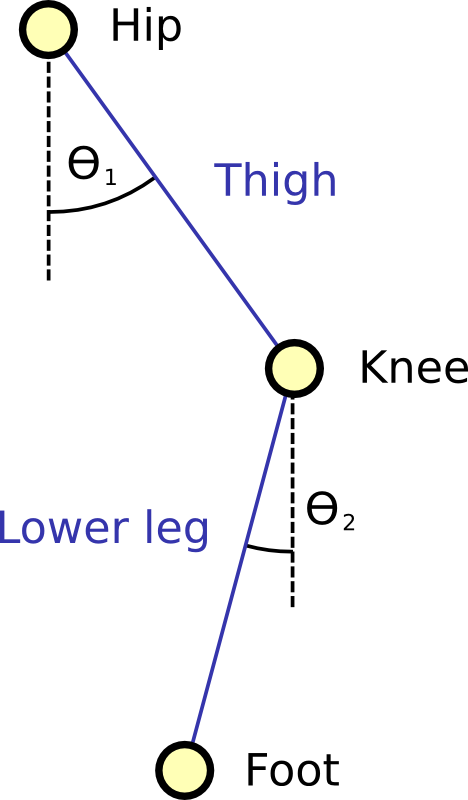
\includegraphics[height=6cm]{model1.png}}
	\qquad
	\subfloat[Front view]{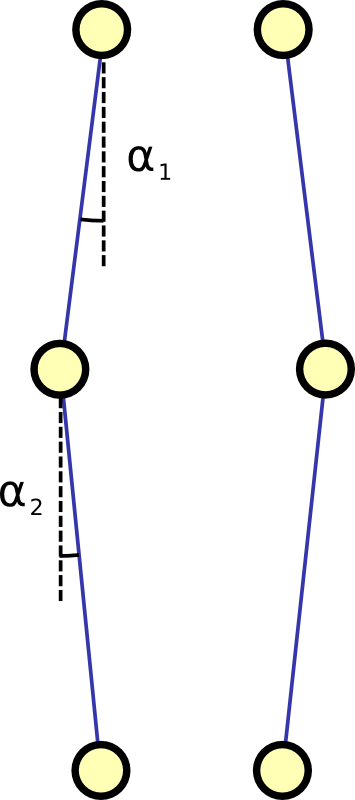
\includegraphics[height=6cm]{model2.png}}
	\caption{Our model for the human leg.}
	\label{ModelImages}
\end{figure}
\clearpage
\section{Cross-correlation}\label{sec:CC}

The first attempt at locating a thigh in the 3D image used the mathematical cross-correlation operator.
A 3D ``thigh-filter'' was generated using Matlab which matched the shape and size of a typical thigh from the sample data.
This was then cross-correlated with the 3D voxel-space image to determine where in the image the thigh was most likely to be.

\bigskip
\noindent Cross-correlation is similar to convolution in that two signals are moved over each other to produce a third signal describing where they best match.
For 3-dimensional discrete input images $f$ and $g$, the cross-correlation image $(f \star g)$ is defined as:

\begin{equation}
	(f \star g)_{(\delta x,\delta y,\delta z)} = \sum_{x=1}^{s_{x}} \sum_{y=1}^{s_{y}} \sum_{z=1}^{s_{z}} f_{(x,y,z)} \cdot g_{(x+\delta x,y+\delta y, z+\delta z)}
\end{equation}

Where $s$ is the size in pixels of the image $f$.

In our case we are not interested in the translation $(\delta x,\delta y,\delta z)$ of the thigh-filter $f$ over the voxel-space image $g$, but rather its rotation.
It is assumed that the thigh has two degrees-of-rotation: $\theta$ - the rotation that makes the leg move in the walking direction, and $\alpha$ - any side-to-side movement of the leg.
We implement this by introducing a transformation matrix $\mathbf{M}(\alpha,\theta)$:

\begin{equation}
	\mathbf{M}(\alpha,\theta) =
	\left(\begin{array}{ccc}
		cos(\alpha) & 0 & sin(\alpha) \\
		0 & 1 & 0 \\
		-sin(\alpha) & 0 & cos(\alpha)
	\end{array} \right)
	\times
	\left(\begin{array}{ccc}
		1 & 0 & 0 \\
		0 & cos(\theta) & -sin(\theta) \\
		0 & sin(\theta) & cos(\theta)
	\end{array} \right)
	\label{eqn:Matrix}
\end{equation}

This allows us to parameterize the cross-correlation image $(f \star g)$ with $\alpha$ and $\theta$ instead:

\begin{equation}
	(f \star g)_{(\alpha,\theta)} = \sum_{x=1}^{s_{x}} \sum_{y=1}^{s_{y}} \sum_{z=1}^{s_{z}} f_{(x,y,z)} \cdot g_{\mathbf{M}(\alpha,\theta) \times (x,y,z)^T}
	\label{eqn:CrossCorrelation}
\end{equation}


\begin{figure}[tb]
	\centering
	\subfloat[Top near hips]{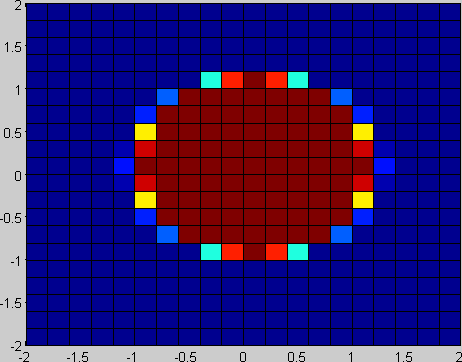
\includegraphics[width=4cm]{../interim/filter1.png}}
	\quad
	\subfloat[Bottom near knees]{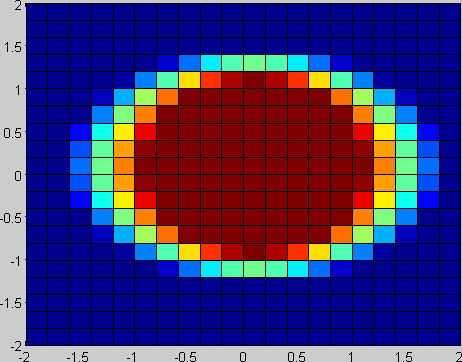
\includegraphics[width=4cm]{../interim/filter2.png}}
	\caption{Cross sections through the 3D thigh-filter.  Red = 1, Blue = 0.}
	\label{ThighFilterCrossSections}
\end{figure}

\bigskip
\noindent The 3D filter is 20x20x20 pixels in volume and generated by a simple Matlab function (see \ref{ThighFilter.m}).
It is exported to a custom binary file format and later loaded by the C code where it is stretched to match the dimensions of the thigh.
Two 2D cross-sections of the filter are shown in Figure \ref{ThighFilterCrossSections}.
From these it can be seen that the filter has a cylindrical core of value 1 to match the solid central section of the thigh.
Additional rings of pixels with lower values are built up around the edge of this cylinder towards the bottom.
The idea is that the filter will then fit ``better'' when it is placed exactly in the center if the thigh,
as this is where the filter pixels with the highest values will correspond to filled voxels in the thigh.

The rings are smaller towards the top of the filter so as not to match the area of filled voxels where the thighs join the hips.

\bigskip
\noindent One of the reasons that this cross-correlation approach was attempted first is that it lends itself very nicely to implementation on a stream processor.
The same matrix multiplications and floating point operations can be performed on a large amount of data at once, with no dependencies or iterative behaviour.
Figure \ref{CrossCorrelation} shows how this is implemented using the OpenGL graphics pipeline.
The fragment shader used is listed in \ref{correlation.cg}.

\begin{figure}[tb]
	\vspace{-10pt}
	\centering
	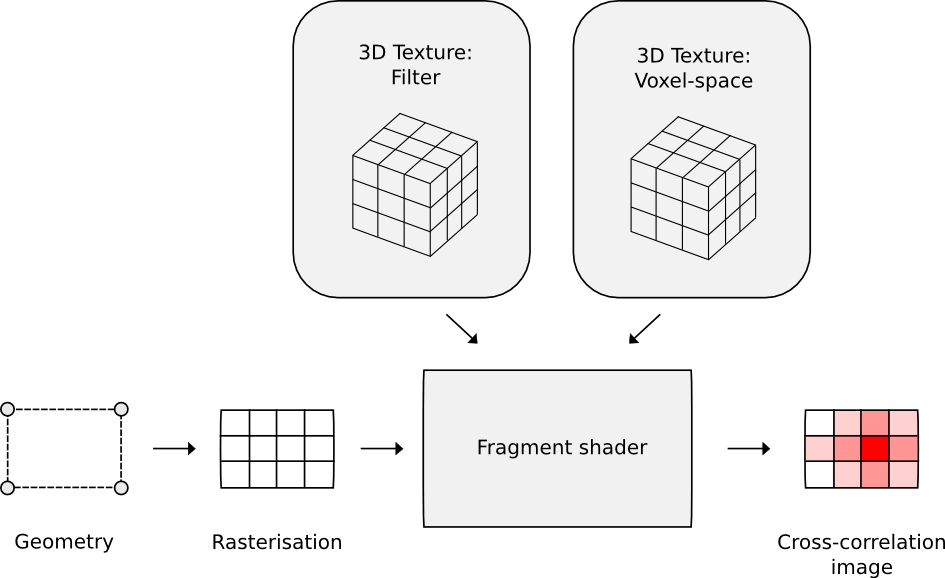
\includegraphics[height=6cm]{../interim/correlation.png}
	\caption{How the OpenGL graphics pipeline can be used to accelerate cross-correlation.
		A quad is drawn and rasterised to match the desired size of the cross-correlation image.
		A fragment program is run on each of the generated fragments to evaluate Equation \ref{eqn:CrossCorrelation}.}
	\label{CrossCorrelation}
\end{figure}

The implementation creates an additional matrix $\mathbf{M}_2$ that is used to convert between the coordinate spaces of OpenGL textures to those of our filters and voxel-space.
It also contains a translate and a scale operation to align the filter with the hips, and scale it to the right size.
The values used in these transformations are obtained from Section \ref{LocatingCenter}.
This $\mathbf{M}_2$ is applied to our original $\mathbf{M}$ from Equation \ref{eqn:Matrix} like so:

\begin{equation}
	\mathbf{M}' = \mathbf{M} \times \mathbf{M}_2
\end{equation}

\bigskip
\noindent The results from this method reveal that perhaps this kind of simple correlation is not suitable for detecting parts of the body in our sample data.
Figure \ref{ParameterSpace} shows the cross-correlation image for a thigh that is oriented straight, in standing position.
It can be seen that $\theta$ is generally correct - horizontally, the concentration of intensity is in the middle of the image, meaning $\theta \simeq 0$.
However vertically there is a far greater concentration of color towards the bottom of the image where $\alpha$ is positive.
This is because here the thigh-filter has been rotated inwards towards the center of the figure, and is matching parts of both left and right legs.

\begin{figure}[tb]
	\vspace{-10pt}
	\centering
	
\includegraphics[height=4cm]{../interim/parameterspace.png}
	\caption{An output cross-correlation image, with correlation strength rendered into the red color channel.
		$\theta$ is mapped to the X axis, and $\alpha$ to Y.
		The center of the image is $(\theta, \alpha) = (0,0)$.}
	\label{ParameterSpace}
\end{figure}

A workaround for this is to fix $\alpha = 0$ and only concern ourselves with $\theta$.
This is acceptable, as the movement of the leg along the walking direction is much greater and more relevant \cite{GaitBook} than its movement perpendicular to that direction.
The results from this method are promising, and demonstrate that the algorithm does work to a certain degree.
\clearpage
\section{Active contours}

Active contours are a useful tool in image processing as they allow a shape to be extracted from potentially noisy data.
It is reasoned that active contours could be used to locate the thigh in a noisy 3D voxel-space reconstruction.
An estimation of the likely position of the thigh is first formed by looking for a concentration of voxels below the hip
(see \ref{LocatingCenter}) and either to the left or right side depending which leg is being located.
Cross-sections of the leg are taken at various heights up the leg, centered around this concentration of voxels - see figure \ref{CrossSections}.
An active contour (or snake) is then placed in the middle of each cross-section and allowed to grow to fill the space available.

\begin{figure}[tb]
	\vspace{-10pt}
	\centering
	\subfloat[Lower legs]{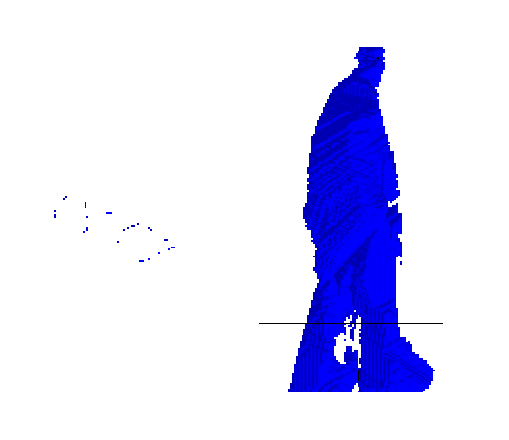
\includegraphics[width=4cm]{../interim/crosssections1.png}}
	\quad
	\subfloat[Thigh joining hips]{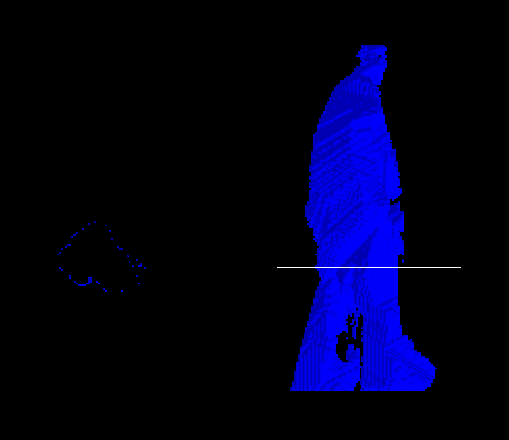
\includegraphics[width=4cm]{../interim/crosssections2.png}}
	\caption{Cross sections taken through the legs at various points (after edge-detection.)}
	\label{CrossSections}
\end{figure}

Hopefully each contour will match the interior area of the thigh at its corresponding height up the leg.
The centers of these contours can then be joined together by a straight line to form the center of the model's cylinder.

As described in section \ref{ContourBackground} an active contour is driven by internal energies and external energies.
A trial-and-error approach was used to generate these energy functions - their effectiveness being tested on a series of artificial images.
The images (see Figure \ref{Contours}) were designed to emulate expected cross-sections of thighs at various heights - ranging from elongated areas
near the hips to closed circular areas further down.
An ideal set of energy functions would cause the contour to match the entire of the closed-area images, but not spread out into
the pelvic area when tested on a cross-section of the joint with the hips.

\begin{figure}[tb]
	\vspace{-10pt}
	\centering
	\subfloat[Inside of thigh]{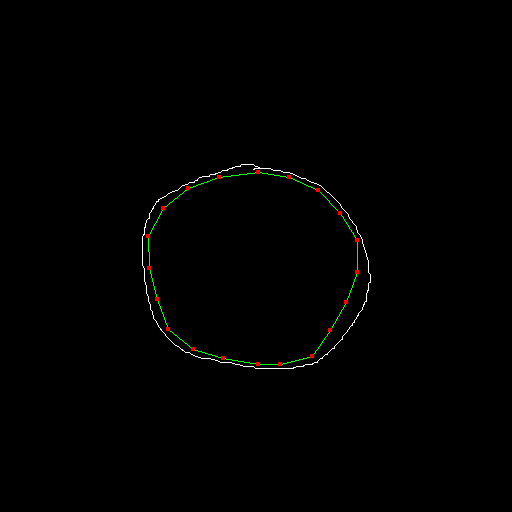
\includegraphics[width=4cm]{../interim/contour2.png}}
	\quad
	\subfloat[Thigh joining hips]{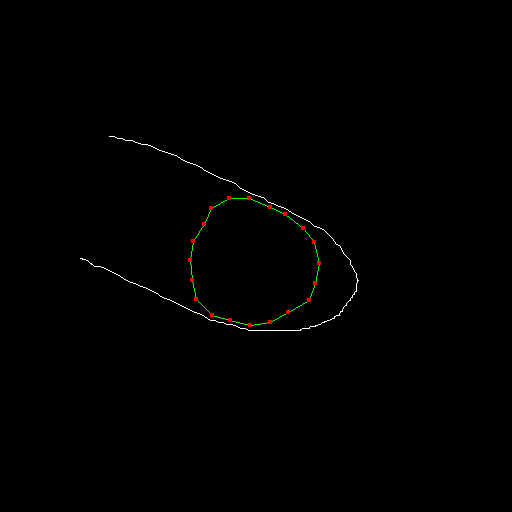
\includegraphics[width=4cm]{../interim/contour4.png}}
	\caption{Snakes matching test images for thigh cross-sections.}
	\label{Contours}
\end{figure}

\bigskip
\noindent A set of four energy functions was created.  It should be noted that in the following equations $n$ is the total number of snaxels,
$\mathbf{V}_{i}$ is the position vector of the snaxel at index $i$ around the contour, where $i \in \{1 \cdots n\}$.
Because the contour is closed all subscript arithmetic is modulo $n$, i.e. $\mathbf{V}_{n+1} = \mathbf{V}_{1}$.
Generally $\mathbf{V}_{i}$ is used to denote the old position of the current snaxel, and $\mathbf{V}_{new}$ its proposed new position
currently being evaluated.

\begin{enumerate}
	\item \textbf{Continuity Energy} - designed to maintain an equal spacing between snaxels.
		\begin{equation}
			E_{cont} = \Bigg| \bigg( \frac{1}{n} \sum_{j=1}^n\| \mathbf{V}_{j-1} - \mathbf{V}_{j} \| \bigg) - \bigg( \| \mathbf{V}_{i-1} - \mathbf{V}_{new} \| \bigg) \Bigg|
		\end{equation}
		This function looks at the difference between the average snaxel spacing and the spacing between the new proposed snaxel and its neighbour.
	
	\item \textbf{Balloon energy} - designed to make the snaxels expand outwards to fill an area.
		\begin{equation}
			E_{bal} = \mathbf{n} \cdot (\mathbf{V}_{i} - \mathbf{V}_{new})
		\end{equation}
		Where $\cdot$ is the inner product operator and $\mathbf{n}$ is the normal unit vector of the snaxel away from the origin position $\mathbf{V}_{origin}$:
		\begin{equation}
			n = \frac{\mathbf{V}_{i} - \mathbf{V}_{origin}}{\|\mathbf{V}_{i} - \mathbf{V}_{origin}\|}
		\end{equation}

	\item \textbf{External energy} - stops the snaxels from crossing filled voxels in the image.
		A filled voxel represents the boundary of the area that the contour should describe, and in its simplest form this function is as follows:
		\begin{equation}
			E_{ext} = I(\mathbf{V}_{new})
		\end{equation}
		Where $I(\mathbf{v})$ is the image intensity at the location $\mathbf{v}$.
		
		A problem with this function is that it is not very robust when there is noise present in the image - the area's edge may have gaps and not be a solid filled line.
		To solve this problem we can sample the image intensity in a 7x7 grid around the location being tested:
		\begin{equation}
			E_{ext} = \sum_{x=-3}^3 \sum_{y=-3}^3 I \binom{\mathbf{V}_{new_0} + x}{\mathbf{V}_{new_1} + y}
		\end{equation}
		This second version has the advantage of overcoming problems that occur when the contour is allowed to jump large numbers of pixels at a time -
		it may occasionally skip over a line in the image completely.
	
	\item \textbf{Shape energy} - ensures the contour stays in a circular shape.
		\begin{equation}
			E_{shape} = \Bigg| \bigg( \frac{2}{n}\sum_{j=1}^n \| \mathbf{V}_{j+\frac{n}{2}} - \mathbf{V}_j \| \bigg) - \bigg( \| \mathbf{V}_{i+\frac{n}{2}} - \mathbf{V}_{new} \| \bigg) \Bigg|
		\end{equation}
		This function depends on there being an even number of snaxels in the contour.
		It works by trying to keep the diameters constant (distances between the current snaxel and the one across the shape from it).
		By doing this we can stop the shape becoming elongated.

\end{enumerate}

\noindent The energy function weights were also chosen by trial-and-error.
The weights that were found to work the best were:
\begin{align*}
	w_{cont} &= 1 \\
	w_{ball} &= 0.3 \\
	w_{shape} &= 0.1 \\
	w_{ext} &= 100
\end{align*}

The overall energy function is therefore given by:

\begin{equation}
	E = w_{cont} E_{cont} + w_{ball} E_{ball} + w_{shape} E_{shape} + w_{ext} E_{ext}
\end{equation}

\bigskip
\noindent The implementation in C of the active contour was fairly straightforward and followed the algorithm given by Williams and Shah \cite{SnakeAlgorithm}.
A \texttt{resetContour} function initialises the contour to a tiny circle at the given location,
and an \texttt{advanceContour} function calculates and updates each snaxel with its next position.
This works by evaluating the energy function at each point in a $k$x$k$ grid centered on the snaxel,
and selecting the one with the lowest value.
The selected point in the grid where the energy function was lowest becomes the snaxel's new position.

This process is repeated until the total change in snaxel position falls below a certain threshold $t$.

Due to its iterative nature it is difficult to find an implementation of this algorithm that is suitable for execution on a stream processor 
However even with a large number of snaxels the C implementation converges on an answer quickly enough for it not to be an issue.

\bigskip
\noindent It is still not certain whether the active contour method is the best way of finding the location of the thigh in an image.
Active contours are generally better suited to locating complex shapes in very noisy greyscale images.
The shape that we are trying to locate here is a simple circle and the values of the pixels in the image are boolean (edge or not-edge).

Perhaps a better approach could be developed by taking some active contour concepts such as internal and external energies,
but restricting the shape to being a perfect circle with a radius $r$ and position $\mathbf{V}$.
This shape would be initialised $r = 0$ and $\mathbf{V} = \mathbf{V}_{origin}$.
Every iteration $r$ would be increased by $1$, and the centre $\mathbf{V}$ moved away from any filled pixels inside the circle's area.
Iteration would cease when the radius could be increased no further without filled pixels appearing on both sides.

This approach would allow the circle to expand and centre itself inside the leg.
It would stop when it could expand no further without breaching the edge of the shape.
\clearpage
\section{3D mesh fitting}

\subsection{Designing a better filter}

The previous approach for cross-correlation described in Section \ref{sec:CC} relies purely on matching filled voxels.
It suffers from the problem that the filter tends to fit better when aligned diagonally across both legs - in the position where it can match the greatest number of voxels.
To correct this problem we can create a new filter that is more intelligent about the type of voxels it matches.

\begin{figure}[b]
	\centering
	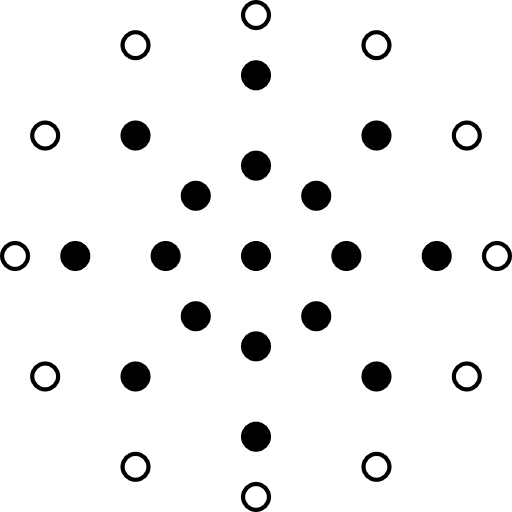
\includegraphics[width=4cm]{../interim/improvedfilter.png}
	\caption{A cross section through the improved cross-correlation filter.
		Black circles represent filled voxels, and white circles represent edge voxels.}
	\label{ImprovedFilterCross}
\end{figure}

Instead of points in the filter having an intensity value $i \in \{0 \cdots 1\}$, our points could take one of two possible states: they could match either an edge voxel or a filled voxel.
This would hopefully overcome the problem of a filter spanning the two legs, as the area between the legs would contain edge voxels.
These edge voxels wouldn't match up with the edge-seeking points in the new filter, and so would be a lower match than if the filter was placed the proper position on the thigh.

\begin{figure}[tb]
	\centering
	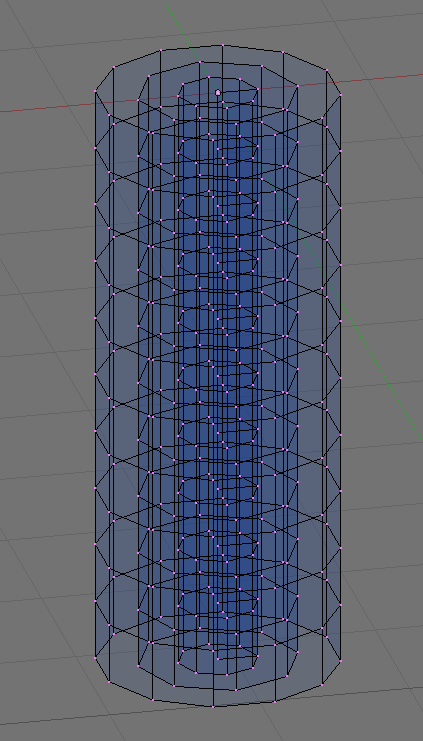
\includegraphics[width=5cm]{thighmodel.png}
	\caption{The cross-correlation filter rendered in the Blender application.
		Although not shown in this image, the outer points in the mesh are coloured white to indicate that they should
		match only edge voxels.}
	\label{ImprovedFilter}
\end{figure}

Figure \ref{ImprovedFilterCross} shows a cross section of such a filter.
It can be seen that the filter contains two types of points - those around the outside that should match edge voxels,
and those in the middle that should match filled voxels through the centre of the thigh.

One important thing to consider about this idea is whether the points in the filter should be spaced in a regular grid.
In the form shown in Figure \ref{ImprovedFilterCross} the points have an arbitrary spacing and are very different from the original filter shown in Figure \ref{ThighFilterCrossSections}.
A filter with points arranged in a regular grid is not necessarily advantageous when matching against discrete voxel data due to the rotations and transformations that the filter will undergo.
In the process of finding the best fitting with the data the filter will be scaled to fit the proportions of the subject, and rotated to match the angle of the leg.
By doing this any one-to-one relationship between pixels in the filter and voxels in the sample data will be lost.

Since there is no advantage to be gained from using a regularly spaced filter, it was decided that a better form for the filter would be that of a mesh.
The final mesh was designed using Blender \cite{Blender} and can be seen in Figure \ref{ImprovedFilter}.



\subsection{Matrix transformations}

In order to match the filter mesh to the voxel data, a matrix would need to be defined that transforms the points from their positions
in mesh-space to their new positions in the voxel-space.
The standard matrix transformations listed in Appendix G of the OpenGL Red Book \cite{RedBook} were used:

\begin{equation}
	\mathbf{M}_{trans}(v) =
	\left(\begin{array}{cccc}
		1 & 0 & 0 & v_{x} \\
		0 & 1 & 0 & v_{y} \\
		0 & 0 & 1 & v_{z} \\
		0 & 0 & 0 & 1
	\end{array} \right)
\end{equation}

\begin{equation}
	\mathbf{M}_{scale}(v) =
	\left(\begin{array}{cccc}
		v_{x} & 0 & 0 & 1 \\
		0 & v_{y} & 0 & 1 \\
		0 & 0 & v_{z} & 1 \\
		0 & 0 & 0 & 1
	\end{array} \right)
\end{equation}

\begin{equation}
	\mathbf{M}_{rotx}(\phi) =
	\left(\begin{array}{cccc}
		1 & 0 & 0 & 0 \\
		0 & cos(\phi) & -sin(\phi) & 0 \\
		0 & sin(\phi) & cos(\phi) & 0 \\
		0 & 0 & 0 & 1
	\end{array} \right)
\end{equation}

\begin{equation}
	\mathbf{M}_{roty}(\phi) =
	\left(\begin{array}{cccc}
		cos(\phi) & 0 & sin(\phi) & 0 \\
		0 & 1 & 0 & 0 \\
		-sin(\phi) & 0 & cos(\phi) & 0 \\
		0 & 0 & 0 & 1
	\end{array} \right)
\end{equation}

\bigskip
First the size of the filter is normalised - scaling all the vertices so they lie in the range ${0 \cdots 1}$.
It is assumed that the origin of the model's coordinate system is already in the centre of its top face.

\begin{equation}
	\mathbf{M}_{1} = \mathbf{M}_{scale}(\frac{1}{\max \{\text{modelSize}_{x}, \text{modelSize}_{y}, \text{modelSize}_{z} \}})
\end{equation}

Then the filter is scaled up to voxel-space.
$h$ is the height of the subject as determined in Section \ref{LocatingCenter}.
We assume that the length of the thighs and lower legs are equal, and are a quarter of the subject's total height.

\begin{equation}
	\mathbf{M}_{2} = \mathbf{M}_{scale}(\frac{h}{4}, \frac{h}{4}, \frac{h}{4})
\end{equation}

Next we apply the relevant rotations to the limbs.
The angles $\theta$ and $\alpha$ used here are the same as in Section \ref{sec:CC} -
$\theta$ is the rotation of the leg along the direction of movement and $\alpha$ is the rotation perpendicular to the direction of movement.

\begin{equation}
	\mathbf{M}_{5} = \mathbf{M}_{rotx}(\theta_{1}) * \mathbf{M}_{roty}(\alpha_{1})
\end{equation}

We now move the mesh to the estimated position of the subject's leg.
Equation \ref{eqn:TransToHip} translates the mesh to the centre of the hip, and equations \ref{eqn:TransToRightLeg} and \ref{eqn:TransToLeftLeg} perform additional
translations to the right or left leg position respectively.
As determined in Section \ref{LocatingCenter} $w$ is the width, or extent along the x axis, of the subject,
and $\mathbf{V}_{mean}$ is the mean filled voxel position.

\begin{align}
	\label{eqn:TransToHip}      \mathbf{M}_{6}  &= \mathbf{M}_{trans}(\mathbf{V}_{mean_{x}}, \mathbf{V}_{mean_{y}}, \frac{h}{2}) \\
	\label{eqn:TransToRightLeg} \mathbf{M}_{7r} &= \mathbf{M}_{trans}(+\frac{w}{6}, 0, 0) \\
	\label{eqn:TransToLeftLeg}  \mathbf{M}_{7l} &= \mathbf{M}_{trans}(-\frac{w}{6}, 0, 0)
\end{align}

Now armed with the above set of transformations, we are able to move the points in our mesh into the correct location in the voxel-space:

\begin{equation}
	\label{eqn:Thigh} \mathbf{M}_{thigh} = \mathbf{M}_{7} * \mathbf{M}_{6} * \mathbf{M}_{5} * \mathbf{M}_{2} * \mathbf{M}_{1}
\end{equation}

You may notice that we have missed out $\mathbf{M}_{3}$ and $\mathbf{M}_{4}$.
Equation \ref{eqn:Thigh} describes the transformation for each of the thighs.
An additional two matrix transformations can be introduced to account for the lower legs:

\begin{align}
	\mathbf{M}_{3} &= \mathbf{M}_{rotx}(\theta_{2}) * \mathbf{M}_{roty}(\alpha_{2}) \\
	\mathbf{M}_{4} &= \mathbf{M}_{trans}(0, 0, -\frac{h}{4})
\end{align}

Again we are using $\alpha$ and $\theta$ to refer to the angles the lower legs make with the vertical.
These equations give us a composite transformation that describes the lower legs:

\begin{equation}
	\label{eqn:LowerLegs} \mathbf{M}_{lowerleg} = \mathbf{M}_{7} * \mathbf{M}_{6} * \mathbf{M}_{5} * \mathbf{M}_{4} * \mathbf{M}_{3} * \mathbf{M}_{2} * \mathbf{M}_{1}
\end{equation}



\subsection{Fitting to the data}

In our previous approach in section TODO, a program would iterate over all the pixels in the filter and sample the
voxel data in the corresponding location.
The value of the filter (a real number between 0 and 1) would be multiplied by the value of the voxel (integer 0 or 1 - representing empty or filled) to produce a ``score''.
The scores of all these samples would then be summed to produce the final fitting score for that orientation.

A better approach would be a more traditional linear regression method such as least squares, as used by Zhihui et al. \cite{LinearModelFitting}.
Figure \ref{FittingImages} shows a two-dimensional example to demonstrate this least squares fitting, however three dimensional fitting works in exactly the same way.
The goal is to fit a mesh (shown as black dashed lines) to voxel data in the shape of a leg (shown as a filled green rectangle).
The mesh contains a number of nodes which are shown in the diagrams as filled circles.
Yellow circles are trying to match edge voxels, and blue circles are trying to match filled non-edge voxels.

\begin{figure}[tb]
	\centering
	\subfloat[High energy fitting]{\label{FittingImageHigh}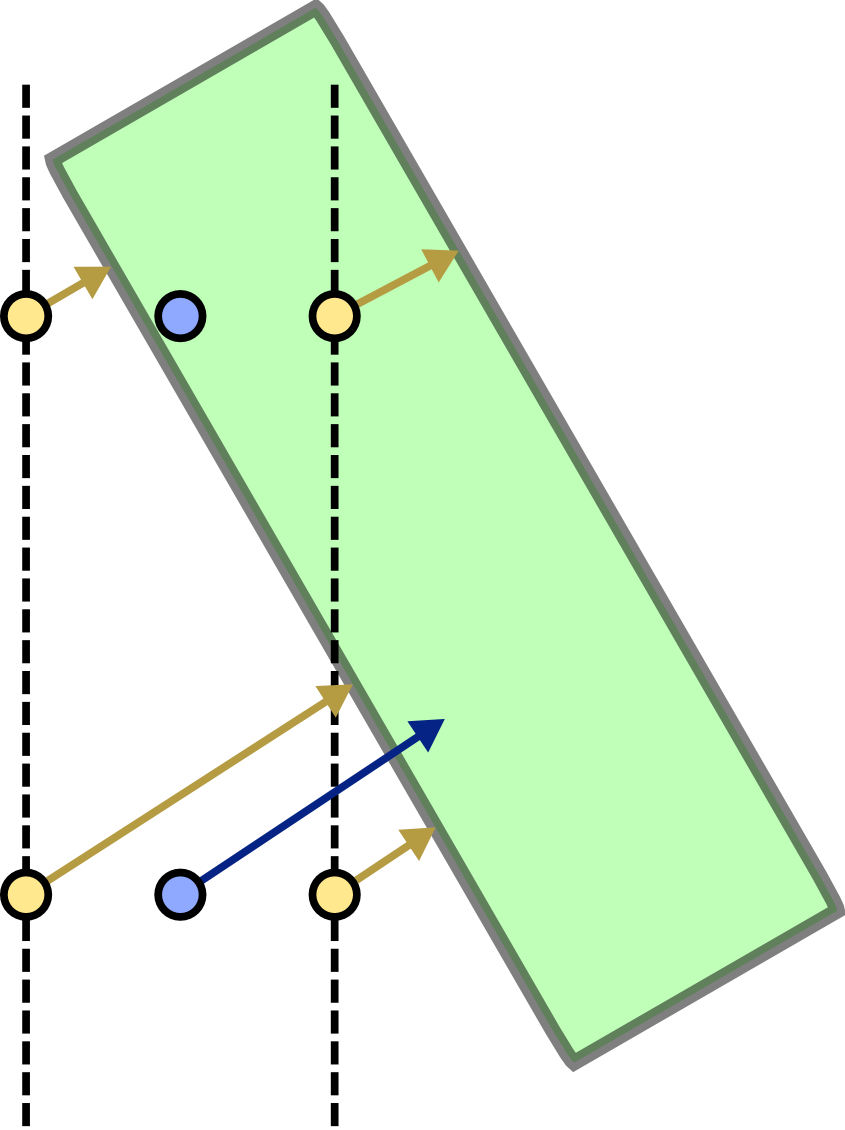
\includegraphics[height=6cm]{fitting1.png}}
	\qquad
	\subfloat[Low energy fitting]{\label{FittingImageLow}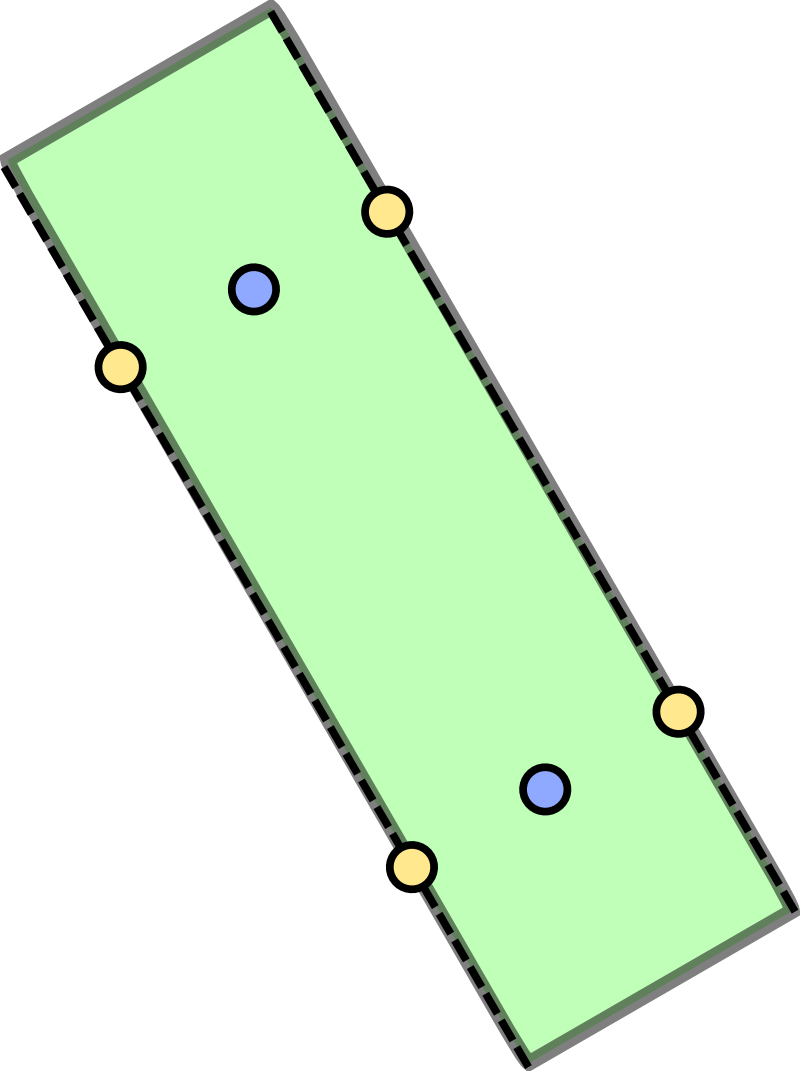
\includegraphics[height=6cm]{fitting2.png}}
	\caption{Potential fittings of our mesh filter.
		The filled green rectangle represents the voxels of a subject's thigh,
		and the coloured circles show a few of the nodes in the mesh.}
	\label{FittingImages}
\end{figure}

An algorithm iterates over the six nodes in the mesh, and for each one searches for the nearest suitable voxel (for the yellow nodes, only edge voxels are suitable).
The first potential fitting, Figure \ref{FittingImageHigh}, has the mesh orientated straight down ($\theta = 0$) and only one of the nodes - the blue one at the top - lies directly on top of a suitable voxel.
The sum of the squared distances between each of the nodes and its closest suitable voxel is taken, and this is used as the overall ``energy'' of that orientation.
Figure \ref{FittingImageHigh} has a high energy as the distances between the nodes and their voxels is very large.
Figure \ref{FittingImageLow} has an energy of $0$, as each node lies directly on top of a suitable voxel.

To find the parameters that give the best fit for an individual frame, one approach would be to iterate over all possible parameters and accept the one that has the least energy.
Such an implementation is shown in Listing \ref{leastsquarescode}.

\begin{lstlisting}[language=c,morekeywords={step,function,foreach,in},frame=single,mathescape=true,caption={Least squares fitting pseudo-code},label={leastsquarescode},float=[tb]]
function fit
	$range_\theta = \frac{\pi}{4}$
	$range_\alpha = \frac{\pi}{32}$
	$resolution_\theta = 41$
	$resolution_\alpha = 11$
	
	$bestEnergy$ = $\infty$
	
	for $\theta_1 = \{-range_\theta \cdots +range_\theta\}$ step $\frac{2range_\theta}{resolution_\theta}$
		for $\theta_2 = \{-range_\theta \cdots +range_\theta\}$ step $\frac{2range_\theta}{resolution_\theta}$
			for $\alpha_1 = \{-range_\alpha \cdots +range_\alpha\}$ step $\frac{2range_\alpha}{resolution_\alpha}$
				for $\alpha_2 = \{-range_\alpha \cdots +range_\alpha\}$ step $\frac{2range_\alpha}{resolution_\alpha}$
					if modelEnergy($\theta_1$, $\theta_2$, $\alpha_1$, $\alpha_2$) < $bestEnergy$
						$bestEnergy$ = modelEnergy($\theta_1$, $\theta_2$, $\alpha_1$, $\alpha_2$)
						$bestParams$ = ($\theta_1$, $\theta_2$, $\alpha_1$, $\alpha_2$)
	
	return $bestParams$

function modelEnergy($params$)
	$energy = 0$
	foreach $node$ in transform($modelMesh$, $params$)
		if isEdgeNode($node$)
			$energy$ += pow(distanceToEdgeVoxel($node$), 2)
		else
			$energy$ += pow(distanceToVoxel($node$), 2)
	
	return $energy$
\end{lstlisting}

We can store the energies at each orientation of the model and use them to plot a graph.
Figure \ref{EnergyPlot} shows the energy for the left thigh in one frame of a sequence.
Note that the search space is actually four-dimensional and hence is difficult to plot on a two-dimensional surface.
In order to visualise the data we have fixed the lower leg parameters ($\alpha_2$ and $\theta_2$) and drawn a slice of $\alpha_1$ against $\theta_1$.

\begin{figure}[tb]
	\centering
	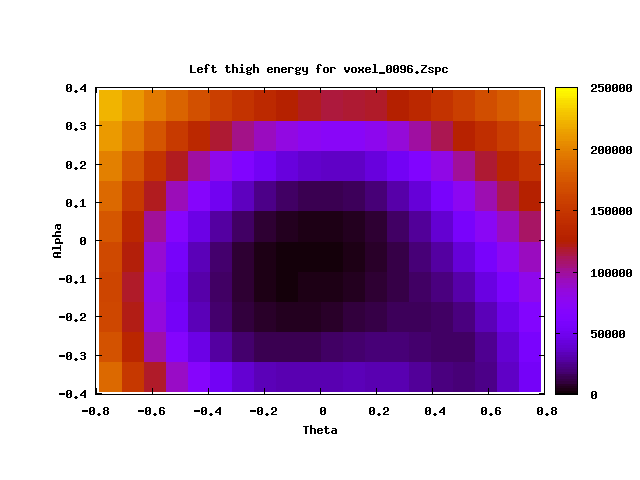
\includegraphics[width=\textwidth]{problems/set81frame96-fixed-leftthigh.png}
	\caption{Energy plot of Frame 96 from Sample 81.
		Darker colours represent lower energies.}
	\label{EnergyPlot}
\end{figure}

We can see from the plot that there is a minimum around the centre - where $(\alpha_1, \theta_1) = (0, 0)$ and the thigh is pointing straight down.

TODO: How do we search for the closest point

\clearpage
\section{Classification}

After every frame in a sample has been through the modelfitting process, we can analyse the sequence as a whole
and produce a series of numbers which describe the subject's gait.
If we are successful, this series of numbers will be unique to each subject and can be used as the basis for classifying any new samples.


\subsection{Extracting a gait cycle}

Before we can perform any kind of analysis on a sample we need to identify and extract one gait cycle.
This is important because we will be comparing different samples which might begin at different times during the subjects' gait cycle.

\begin{figure}[tb]
	\centering
	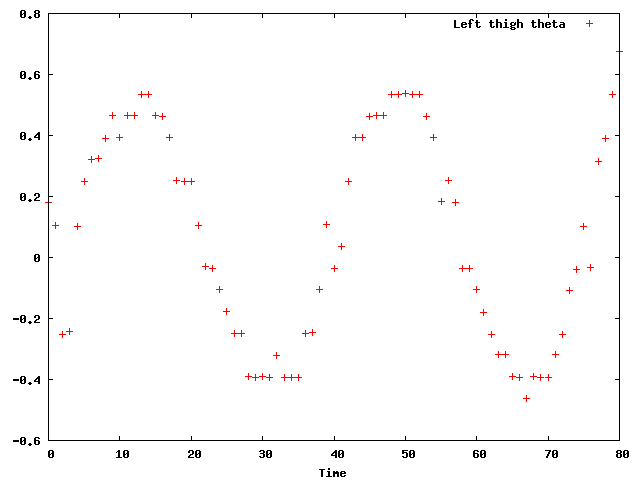
\includegraphics[width=\textwidth]{curvefitting.png}
	\caption{The change in $\theta_1$ over time for Sample 81.}
	\label{CurveFitting1}
\end{figure}

Figure \ref{CurveFitting1} shows a typical plot of the change in the value of $\theta_1$ over time.
The graph resembles a sinosoid which we intuitavely know to be correct - when we walk our thighs swing forwards and backwards like a pendulum.
A gait cycle is usually defined as beginning and ending with heel strikes of the same foot (TODO: citation), which in Figure \ref{CurveFitting1} would be two subsequent maximums of the sinosoid.
We however are going to begin our gait cycle when the thigh crosses the vertical, ie. when $\theta = 0$.

We can find this point where the thigh crosses the vertical by fitting a function $f_1(t)$ to our data points and finding where $f_1(t) = 0$.
The function we use is shown in Equation \ref{eqn:CurveFitting}:

\begin{equation}
	f_1(t) = d + a \sin(\frac{2 \pi t}{\xi} + \phi)
	\label{eqn:CurveFitting}
\end{equation}

The DC offset, $d$, and amplitude, $a$, were found to be fairly similar for all subjects, so were kept fixed at $d = 0.05$ and $a = 0.55$.
Least squares regression was used to find the values for $\xi$, the period of the gait cycle, and $\phi$, the phase offset.

\begin{figure}[tb]
	\centering
	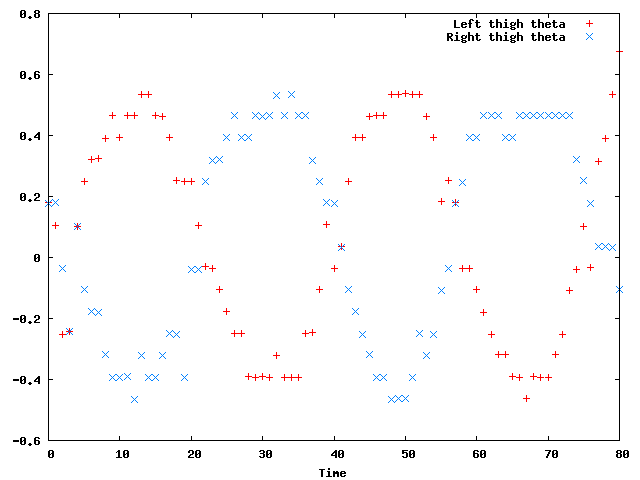
\includegraphics[width=\textwidth]{curvefitting2.png}
	\caption{The change in $\theta_1$ and $\theta_2$ over time for Sample 81.
		The two parameters are $90^\circ$ out of phase.}
	\label{CurveFitting2}
\end{figure}

Equation \ref{eqn:CurveFitting} above describes the general motion of only one of the thighs.
We can increase accuracy by including the motion of the other thigh as well.
We make use of the observation that the motion of the two thighs are $90^\circ$ out of phase (see Figure \ref{CurveFitting2}):

\begin{equation}
	f_2(t) = d + a \sin(\frac{2 \pi t}{\xi} + \phi + \pi)
	\label{eqn:CurveFitting2}
\end{equation}

The implementation used for our least squares fitting is similar to that in Listing \ref{leastsquarescode}, however instead of looking over a four-dimensional parameter space we are only interested in $\xi$ and $\phi$.
The ranges used for these variables are $\xi = [30, 40]$ and $\phi = [0, 2\pi]$.
The assumption that the period of one gait cycle lies in this range $[30, 40]$ was arrived at by observation of the typical gait cycles in our database.

The energy function used to determine the suitability of each set of parameters is worth mentioning as it has to take into account two curves and two sets of data.
It is shown in Listing \ref{curvefittingenergy}.
This function is used in a similar way to $modelEnergy$ in Listing \ref{leastsquarescode}.

\begin{lstlisting}[firstnumber=1,language=c,morekeywords={step,function,foreach,in},frame=single,mathescape=true,caption={Energy function pseudo-code},label={curvefittingenergy},float=[tb]]
function energy($\xi$, $\phi$)
	$d = 0.05$
	$a = 0.55$
	
	$energy = 0$
	foreach $t$
		$expected_{left} = d + a \sin(\frac{2 \pi t}{\xi} + \phi)$
		$expected_{right} = d + a \sin(\frac{2 \pi t}{\xi} + \phi + \pi)$
		$actual_{left}$ = $\theta_1$[$t$]
		$actual_{right}$ = $\theta_2$[$t$]
		
		$energy$ += $(expected_{left} - actual_{left})^2$
		$energy$ += $(expected_{right} - actual_{right})^2$
	
	return $energy$
\end{lstlisting}

Once we have obtained values for $\xi$ and $\phi$ we can find the time $z$ of each zero-crossing like so:

\begin{equation}
	z_i = \frac{\xi \sin^{-1}(-\frac{d}{a} - \phi)}{2\pi} + i\pi
\end{equation}


\subsection{Discrete fourier transforms}

Now that we can extract a gait cycle from each sample we need to apply the DFT (Discrete Fourier Transform) to them to obtain information about the frequency components of the subject's gait.
Previous work (TODO: citations) have suggested that these frequency components can be used to form an identifying signature for the subject.

\begin{equation}
	X_i = \sum_{n=0}^{N-1} x_n e^{-\frac{2 \pi i}{N} i n} \quad \quad i = 0, \dots, N-1
\end{equation}


What does it do?

Implementation: FFTW library \cite{FFTW}
Assume that there's one period and the start is free of noise.  Ref set 4.

\subsection{Classification methods}
Show details of different classification approaches.
Graphs in complex plane to determine distance.

Take the polar distance instead!


\chapter{Results}

\section{Accuracy of modelfitting}

\subsection{Ranges and resolutions}

One of the major problems faced throughout the development of the modelfitting algorithm was with the selection of ranges and resolutions.
In Listing \ref{leastsquarescode} there is a mention of four variables - $range_\theta$, $range_\alpha$, $resolution_\theta$ and $resolution_\alpha$.
These variables control the size and resolution of the parameter space that is searched during the modelfitting.
Care must be taken when adjusting these variables as they control both the accuracy of the results and the execution time of the algorithm.

Some of the problems encountered when selecting values for the variables are given below.

\begin{figure}[p]
	\centering
	\subfloat[Left thigh energy]{\label{Alpha:GoodLeftThigh}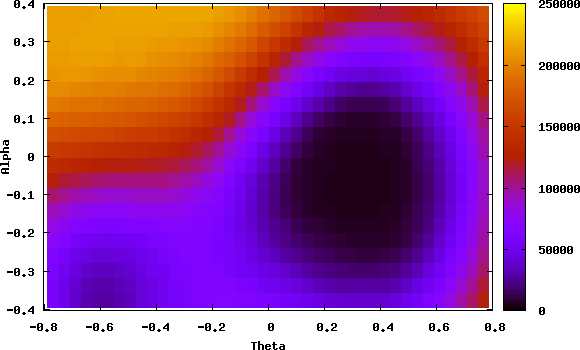
\includegraphics[width=6.2cm]{problems/good-leftthigh.png}}
	\qquad
	\subfloat[Right thigh energy]{\label{Alpha:GoodRightThigh}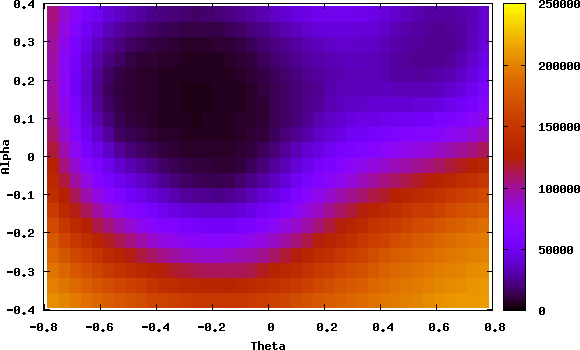
\includegraphics[width=6.2cm]{problems/good-rightthigh.png}}
	\\
	\subfloat[Left lower leg energy]{\label{Alpha:GoodLeftLower}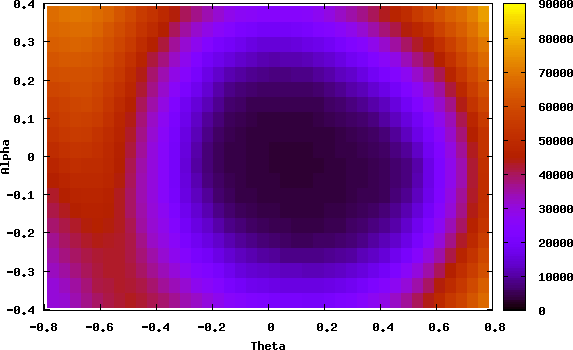
\includegraphics[width=6.2cm]{problems/good-leftlower.png}}
	\qquad
	\subfloat[Right lower leg energy]{\label{Alpha:GoodRightLower}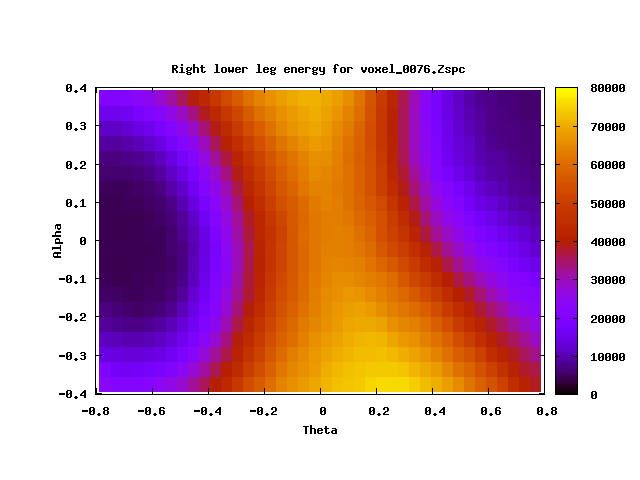
\includegraphics[width=6.2cm]{problems/good-rightlower.png}}
	\\
	\subfloat[Model and voxel data]{\label{Alpha:Good3D}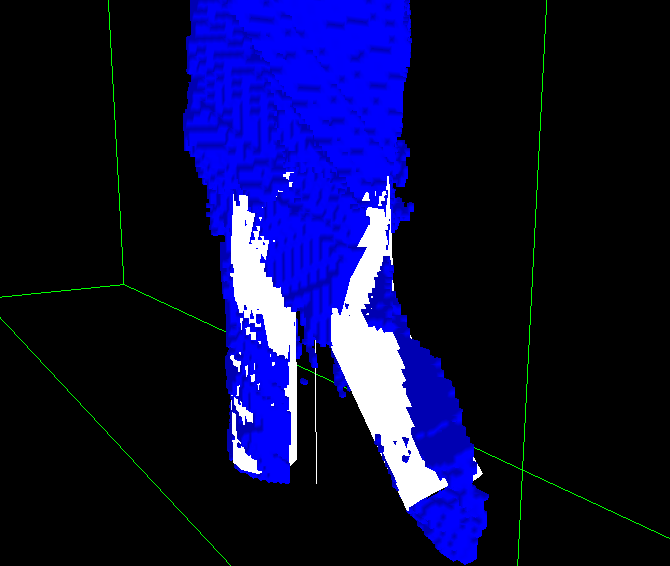
\includegraphics[width=6.2cm]{problems/good-3d.png}}
	\qquad
	\subfloat[Model]{\label{Alpha:GoodModel}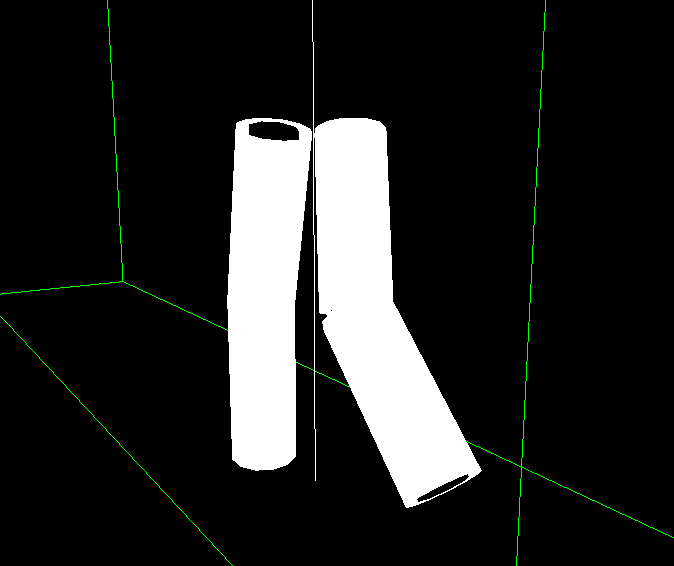
\includegraphics[width=6.2cm]{problems/good-model.png}}
	
	\caption{Frame 76, a good fitting of the model to the data.
		Notice in \ref{Alpha:GoodRightThigh} how there is a local minimum developing in the upper-right corner.
		Remember that \ref{Alpha:GoodRightThigh} and \ref{Alpha:GoodRightLower} are slices through a four-dimensional space,
		and as such there may be minima elsewhere that are not shown.}
	\label{AlphaGood}
\end{figure}

\begin{figure}[p]
	\centering
	\subfloat[Left thigh energy]{\label{Alpha:BadLeftThigh}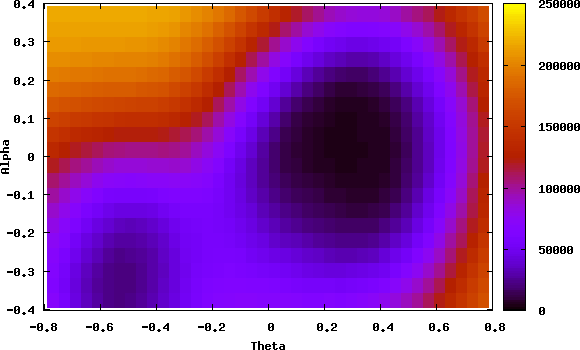
\includegraphics[width=6.2cm]{problems/badalpha-leftthigh.png}}
	\qquad
	\subfloat[Right thigh energy]{\label{Alpha:BadRightThigh}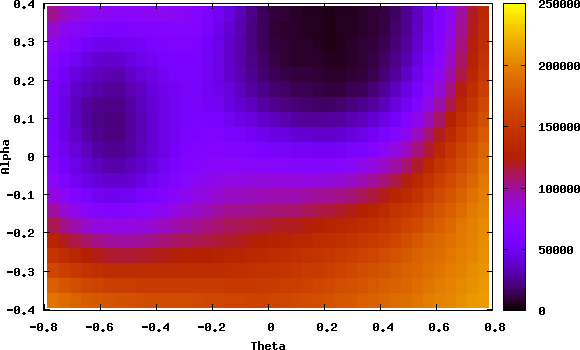
\includegraphics[width=6.2cm]{problems/badalpha-rightthigh.png}}
	\\
	\subfloat[Left lower leg energy]{\label{Alpha:BadLeftLower}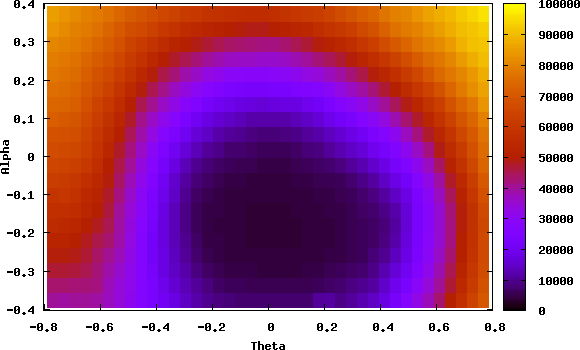
\includegraphics[width=6.2cm]{problems/badalpha-leftlower.png}}
	\qquad
	\subfloat[Right lower leg energy]{\label{Alpha:BadRightLower}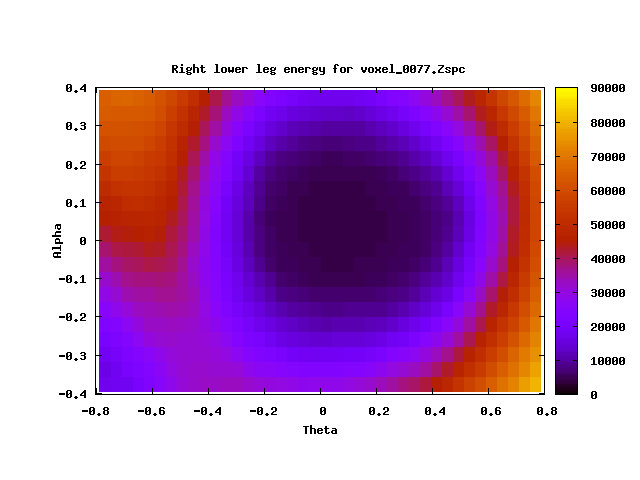
\includegraphics[width=6.2cm]{problems/badalpha-rightlower.png}}
	\\
	\subfloat[Model and voxel data]{\label{Alpha:Bad3D}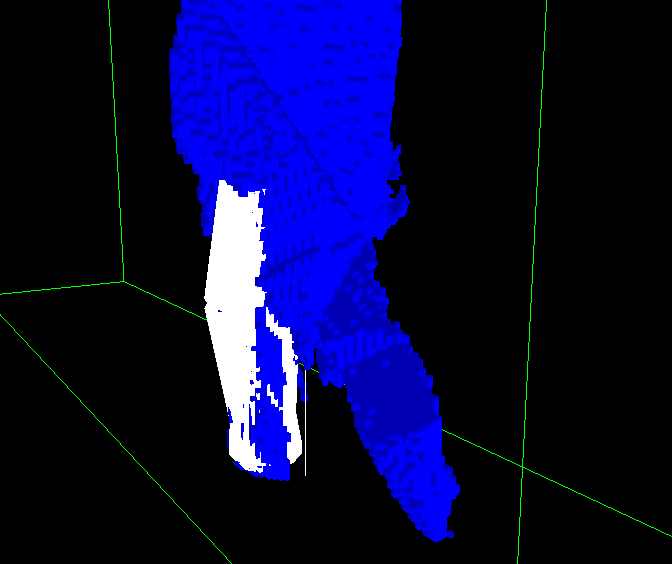
\includegraphics[width=6.2cm]{problems/badalpha-3d.png}}
	\qquad
	\subfloat[Model]{\label{Alpha:BadModel}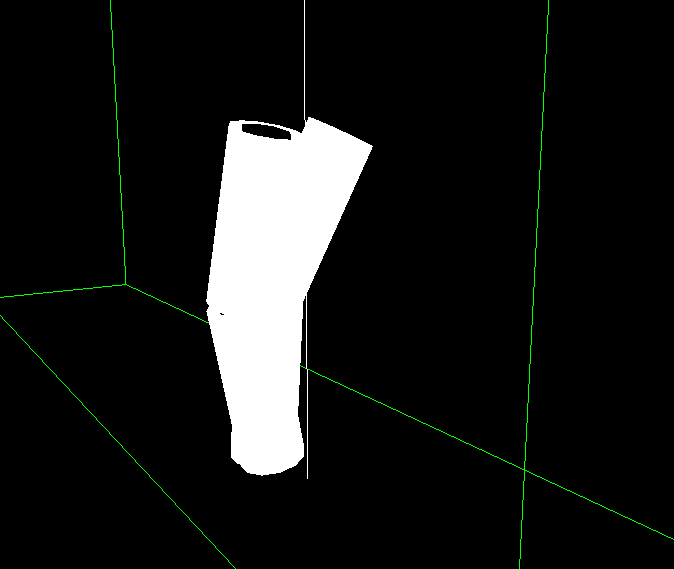
\includegraphics[width=6.2cm]{problems/badalpha-model.png}}
	
	\caption{Frame 77, an erroneous fitting of the model to the data.
		The local minimum in \ref{Alpha:GoodRightThigh} on the previous page must have had a much lower energy with $(\alpha_2, \theta_2) = (0, 0)$ (lower leg energy).
		In this frame the energy at that point became even lower - lower than that of the correct point - and became the global minimum.}
	\label{AlphaBad}
\end{figure}

\begin{enumerate}
	\item \textbf{Erroneous minima}.
		Originally we had set $range_\alpha = \left[ -\frac{\pi}{8}, +\frac{\pi}{8}\right]$.
		This range turned out to be far too big, and as such would lead to erroneous minima being found.
		The problem tended to occur when the two thighs were close together - one of the thighs would assume
		a large alpha value and swing towards the subject's other leg.
		The two leg models would then intersect as they matched the same leg in the data.
		
		Figures \ref{AlphaGood} and \ref{AlphaBad} demonstrate this problem.
		They are of subsequent frames in sample 81 - the first frame matches the right leg correctly
		but the second frame is incorrect.
		The right thigh has an alpha value that is strongly positive, and this leads to it matching most of the left leg instead.
		
		To understand why this has happened we need to remember that the parameter space is four-dimensional, and each of the energy plots
		shown are only slices with two of the parameters held constant.
		Therefore much of the parameter space is not shown in the plots.
		Figure \ref{Alpha:GoodRightThigh} shows a small low energy region near the top, in a similar location to the larger low energy region in Figure \ref{Alpha:BadRightThigh}.
		The energy of this region in the first plot is not nearly as low as the other, correct, minimum, so we may wonder why it has grown so dramatically between frames.
		The answer is that Figure \ref{Alpha:GoodRightThigh} is a slice at the minimum in Figure \ref{Alpha:GoodRightLower} - if we moved it so the slice
		were instead taken at the minimum from Figure \ref{Alpha:BadRightLower} we would likely see a much stronger low energy region.
		
		This was a major problem, and a number of approaches were taken to attempt to solve it.
		The first was to smooth the data - using the results of the previous frames to apply a penalty to parameters that were too far away from the expected position.
		However this seemed more like a remedy to the result of the problem (wrong minima being chosen) rather than the cause of it (bad alpha range).
		Also it was feared that any kind of smoothing of the data might destroy valuable gait information.
		
		Instead it was decided to take the simpler solution - limiting the range of possible alpha values.
		A strong divide was noted between the typical alpha values of correct and incorrect frames - the correct frames all took on
		values within the range $\left[ -\frac{\pi}{32}, +\frac{\pi}{32}\right]$, and the others outside.
		$range_\alpha$ was therefore set to $\left[ -\frac{\pi}{32}, +\frac{\pi}{32}\right]$.
	
	\item \textbf{Oversampling}.
		There is a limit to the maximum resolution at which it is sensible to sample the parameter space.
		The size of the voxels in the data is $1\text{cm}^3$.
		Comparing the fitting of two orientations of the model that differ by less than $1\text{cm}^3$ is meaningless,
		as the coordinates of every distance lookup performed are clamped to integer values (not doing so would break
		the lookup cache from section TODO).
		
		Sampling at these high resolutions could not be considered before multi-resolution sampling (TODO) was implemented
		as the execution time would have been prohibitive.
		With the introduction of multi-resolution sampling however some high-resolution fittings were tested, and as expected
		the noise resulting from the discrete nature of the data led to errors in the DFT and a lower classification rate.
		
		The ideal resolutions were discovered to be $resolution_\theta = 41$ and $resolution_\alpha = 11$ - meaning the
		parameter space is 41x41x11x11 (odd numbers were chosen to ensure there is one sample taken at $(0, 0, 0, 0)$).
\end{enumerate}


\subsection{Quantitative error analysis}

A manual fitting was produced for selected samples to provide a means of evaluating the error of the modelfitting algorithm.
Each frame was examined in the modelfitting application, and the parameters of the model tweaked to visually fit the model to the image of the subject.
Samples 81 and 96 were chosen for this manual fitting process as they gave very different success rates in classification.
Sample 81 is one of the samples of Subject 1, who was classified correctly in most of the tests.
Sample 96 is one of the samples of Subject 4, who was never classified correctly in any of the tests.

Figures \ref{ManualFit81} and \ref{ManualFit96} show the differences between parameter values for automatic fitting and manual fitting,
and Figures \ref{ManualFitTable81} and \ref{ManualFitTable96} summarise these results in tabular form.
Only the $\theta$ values were compared as their errors affect classification far more than those in the $\alpha$ values.

In the tables below $a_t$ represents the value of $\theta$ that was determined automatically, and $m_t$ the value that was entered manually.

\begin{figure}[thb]
	\begin{center}
		\begin{tabular}{l|c|c|c|c}
			& $\sum_{t=1}^N \left| a_t - m_t \right|$ & $\frac{\sum_{t=1}^N \left| a_t - m_t \right|}{N}$ & $\sum_{t=1}^N \left( a_t - m_t \right)^2 $ & $\frac{\sum_{t=1}^N \left( a_t - m_t \right)^2}{N}$ \\
			\hline
			Left thigh & 2.38639 & 0.0294616 & 0.371018 &0.00458047 \\
			Right thigh & 1.76716 & 0.0218168 & 0.206641 &0.00255113 \\
			Left lower & 4.33182 & 0.0534793 & 1.58659 &0.0195875 \\
			Right lower & 2.56525 & 0.0316698 & 0.540861 &0.0066773 \\
			\hline
			Total & 11.0506 & 0.136427 & 2.70511 & 0.0333964 \\
		\end{tabular}
	\end{center}
	\caption{Error between automatic and manual fittings for Sample 81.}
	\label{ManualFitTable81}
\end{figure}

\begin{figure}[thb]
	\begin{center}
		\begin{tabular}{l|c|c|c|c}
			& $\sum_{t=1}^N \left| a_t - m_t \right|$ & $\frac{\sum_{t=1}^N \left| a_t - m_t \right|}{N}$ & $\sum_{t=1}^N \left( a_t - m_t \right)^2 $ & $\frac{\sum_{t=1}^N \left( a_ t- m_t \right)^2}{N}$ \\
			\hline
			Left thigh & 0.15711 & 0.00285655 & 0.0131091 &0.00023835 \\
			Right thigh & 0.667605 & 0.0121383 & 0.0979246 &0.00178045 \\
			Left lower & 0.137471 & 0.00249947 & 0.018892 &0.00034349 \\
			Right lower & 1.64081 & 0.0298329 & 0.434485 &0.00789972 \\
			\hline
			Total & 2.603 & 0.0473272 & 0.56441 & 0.010262 \\
		\end{tabular}
	\end{center}
	\caption{Error between automatic and manual fittings for Sample 96.}
	\label{ManualFitTable96}
\end{figure}

\begin{figure}[p]
	\centering
	\subfloat[Left thigh]{\label{ManualFit81:LeftThigh}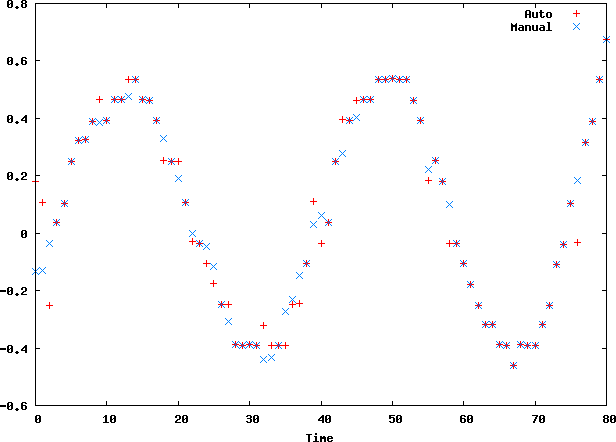
\includegraphics[width=6.2cm]{manualfitting/81-leftthightheta.png}}
	\quad
	\subfloat[Right thigh]{\label{ManualFit81:RightThigh}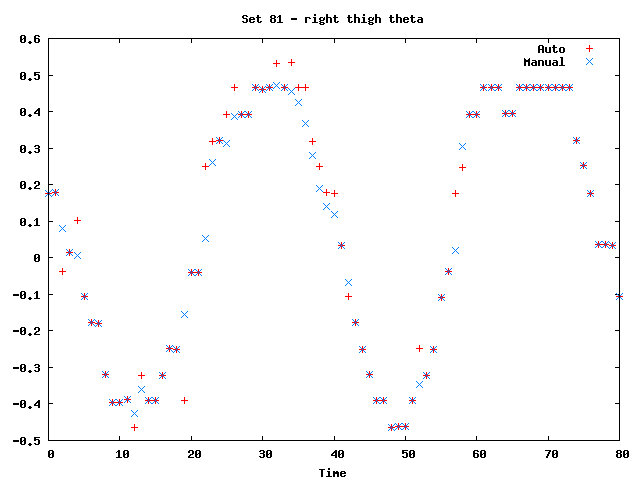
\includegraphics[width=6.2cm]{manualfitting/81-rightthightheta.png}}
	\\
	\subfloat[Left lower leg]{\label{ManualFit81:LeftLower}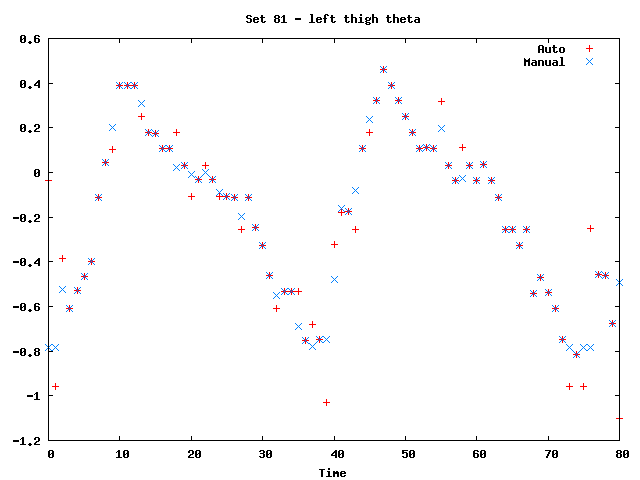
\includegraphics[width=6.2cm]{manualfitting/81-leftlowertheta.png}}
	\quad
	\subfloat[Right lower leg]{\label{ManualFit81:RightLower}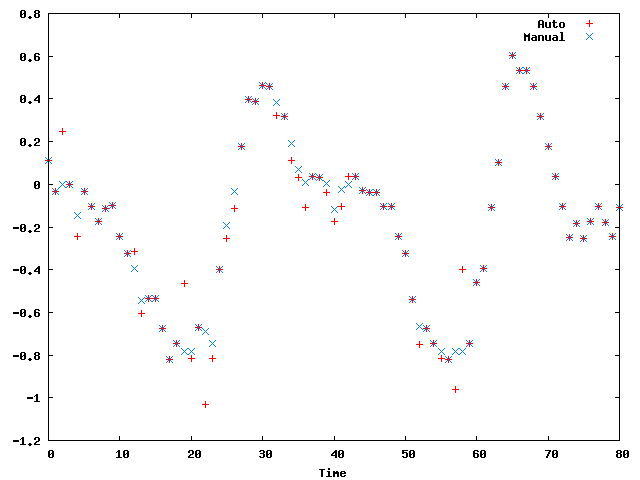
\includegraphics[width=6.2cm]{manualfitting/81-rightlowertheta.png}}
	
	\caption{Comparison between automatic and manual fittings for Sample 81.}
	\label{ManualFit81}
\end{figure}

\begin{figure}[p]
	\centering
	\subfloat[Left thigh]{\label{ManualFit96:LeftThigh}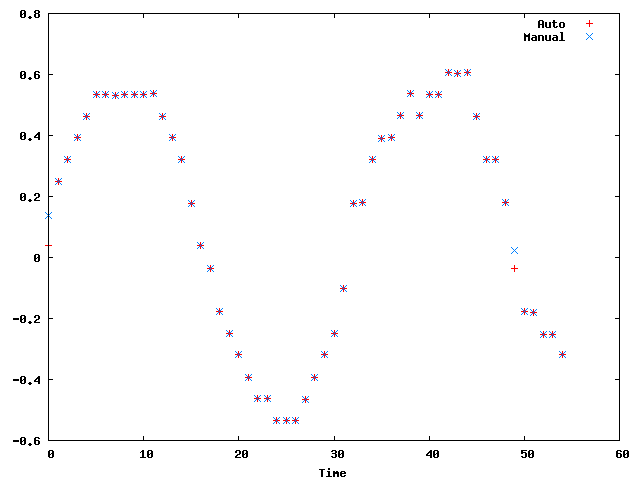
\includegraphics[width=6.2cm]{manualfitting/96-leftthightheta.png}}
	\quad
	\subfloat[Right thigh]{\label{ManualFit96:RightThigh}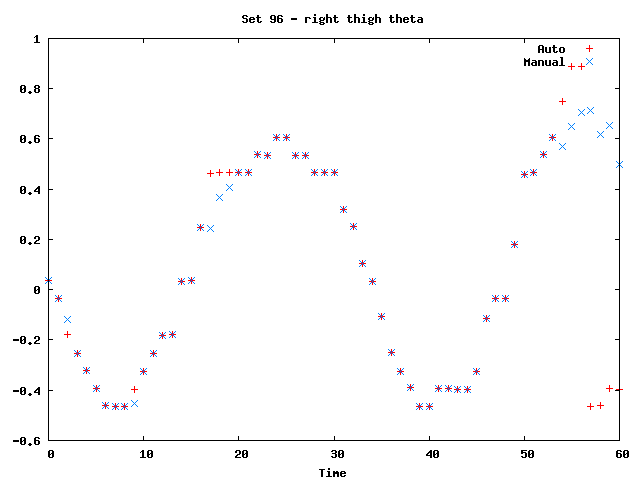
\includegraphics[width=6.2cm]{manualfitting/96-rightthightheta.png}}
	\\
	\subfloat[Left lower leg]{\label{ManualFit96:LeftLower}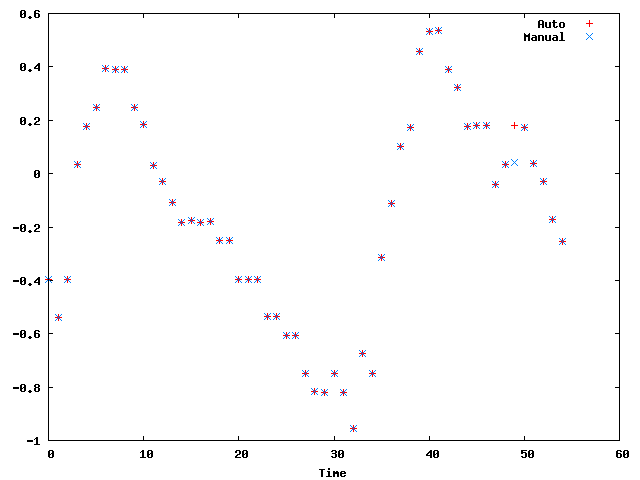
\includegraphics[width=6.2cm]{manualfitting/96-leftlowertheta.png}}
	\quad
	\subfloat[Right lower leg]{\label{ManualFit96:RightLower}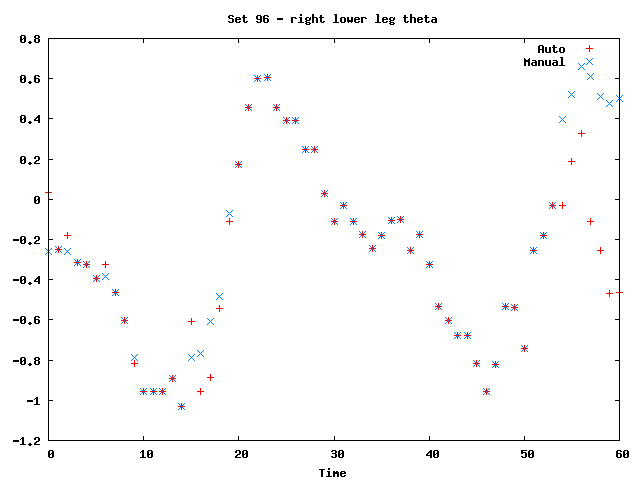
\includegraphics[width=6.2cm]{manualfitting/96-rightlowertheta.png}}
	
	\caption{Comparison between automatic and manual fittings for Sample 96.}
	\label{ManualFit96}
\end{figure}

TODO: Analysis of the numbers - why is 96 ``better'' than 81 - maybe it was the other samples in the set that were wrong?

TODO: Suggest why they might be bad - noise.

\clearpage
\section{Accuracy of classification}

In the previous chapters we have presented a selection of different algorithms and approaches to modelfitting and classification.
This section attempts to discover which combination of these algorithms leads to the best performance in terms of recognising new subjects.

The sample data used to test the algorithms contains 10 different subjects.
Four recordings of each subject were taken, giving a total of 40 samples.
Two of the four samples from each subject were manually classified and entered into a database for use as a training set,
while the remaining two samples (labelled \emph{a} and \emph{b}) were put through automatic classification.

The success rate of the system was determined by how many of the ``unknown'' samples \emph{a} and \emph{b} it was able to match to the correct class in the training set.
In the tables below (\ref{ClassificationResults} and \ref{ClassificationResults2}) the numbers in each cell represent how close the algorithm came to correctly identifying the subject.
A value of 3 would indicate that there were 3 other classes that were a better match than the correct one,
while a value of 0 would represent a correct classification.

\bigskip
\noindent There were four primary questions that guided the testing process:

\begin{enumerate}
	\item \textbf{Which distance function is most suitable?}
		Section \ref{ClassificationMethods} described some of the possible \emph{distance functions} that could be implemented to find how closely related two samples are to each other.
		These functions take the results of the DFT as applied to both of the samples and compare each of the frequency components.
		Table \ref{ClassificationResults} over the page shows the performance of each of these functions.
		
		First we test the basic distance functions.
		Four such functions are tested - one that compares only the magnitudes of the frequency components, one that compares the phase weighted magnitudes, and two that take the polar and euclidean distances between two frequency components in the complex plane.
		From the results we can see that the highest performers are the polar and euclidean distance functions.
		The low performance of the phase-weighted magnitude function can be explained by the fact that it does not take into account the modular nature of the phase.
		As explained in Section \ref{ClassificationMethods} a comparison of two phase values $+\frac{5}{6}\pi$ and $-\frac{5}{6}\pi$ would incorrectly produce an answer of $\frac{10}{6}\pi$.
		
		Next all the functions are retested with the first frequency component of each sample being excluded.
		The results show that this actually lowers the performance of all the functions - suggesting that the first frequency component might contain useful identifying information.
		
		The euclidean distance function is then modified to normalise the mean of the samples' DFT results.
		This does indeed improve the performance - increasing the correct classification rate by 5\%.
	
	\item \textbf{Which of the search algorithms are best?}
		We started off by introducing a fixed resolution search in Listing TODO, and then later attempted to lower its execution time by splitting it into two passes.
		It is important to evaluate both these fixed and multi-resolution search algorithms in order to ensure that we are not sacrificing performance for speed of execution.
		
		Three algorithms were tested - a fixed resolution search with a low resolution ($\text{res}_\alpha = 11, \text{res}_\theta = 21$),
		a fixed resolution search with a high resolution ($\text{res}_\alpha = 11, \text{res}_\theta = 41$),
		and a multi-resolution search (with equivalent $\text{res}_\alpha = 41, \text{res}_\theta = 81$).
		The results from these tests are shown in Table \ref{ClassificationResults2}.
		
		Suprisingly, these tests show that the best performer is the low fixed-resolution search algorithm.
		Using this algorithm we can correctly classify 80\% of all the test subjects.
		Both the high resolution and multi resolution algorithms seem to have much lower performance - demonstrating a lower overall classification rate.
		However if we look at the distances between our sample and the nearest sample of the correct class we can see that they are still very close - the higher resolution searches
		have just moved a sample of another class a little bit closer, throwing off the classification.
		
	\item \textbf{Which limbs are important in classification?}
		Our initial tests in Table \ref{ClassificationResults} were performed using only the signature data from the subject's left thigh.
		In Table \ref{ClassificationResults2} we run additional tests to see if there is any improvement to be gained from including the right thigh and lower legs.
		
		Using both thighs in classification gives an improvement over just using the left thigh - one additional sample is classified correctly bringing the success rate up from 75\% to 80\%.
		
		Including the lower legs brings about a drop in performance of 10\%-20\% over all the search algorithms, so clearly these are less useful than the thighs for identification.
		Using \emph{both} thighs and lower legs seems to bring us to a middle ground in classification performance - 65\% of the samples being classified correctly.
	
	\item \textbf{Can the subject's height be used for classification?}
		The final test performed was to find out whether including the subject's height as an additional classifier would boost performance.
		
		Figure \ref{ClassificationResults2} shows that including the height provides a huge boost in performance, bringing the overall success rate up to 90\%.
		Interestingly this was the only test that correctly classified Sample 10b.
\end{enumerate}

\begin{landscape}
	\begin{table}[p]
		\centering
		\begin{tabular}{|l|c@{ }c|c@{ }c|c@{ }c|c@{ }c|c@{ }c|c@{ }c|c@{ }c|c@{ }c|c@{ }c|c@{ }c|c|}
			\hline
			& \multicolumn{20}{|c|}{Sample} & Success rate \\
			& 1a & 1b & 2a & 2b & 3a & 3b & 4a & 4b & 5a & 5b & 6a & 6b & 7a & 7b & 8a & 8b & 9a & 9b & 10a & 10b & \\
			
			\hline
			Magnitude                  & 1 & 2 & 1 & 0 & 0 & 1 & 6 & 11 & 4 & 0 & 3 & 0 & 0 & 2 & 0 & 0 & 1 & 2 & 2 & 0 & 40\% \\
			Phase-mag                  & 0 & 2 & 0 & 6 & 0 & 1 & 12 & 10 & 3 & 3 & 0 & 4 & 1 & 0 & 0 & 2 & 10 & 16 & 1 & 5 & 30\% \\
			Polar dist                 & 0 & 3 & 0 & 0 & 0 & 0 & 0 & 11 & 0 & 3 & 2 & 0 & 0 & 0 & 0 & 0 & 7 & 0 & 0 & 16 & 70\% \\
			Eucl dist                  & 0 & 3 & 0 & 0 & 0 & 0 & 0 & 11 & 0 & 3 & 2 & 0 & 0 & 0 & 0 & 0 & 7 & 0 & 0 & 16 & 70\% \\
			
			\hline
			Mag excl first             & 2 & 1 & 1 & 6 & 1 & 1 & 0 & 2 & 14 & 2 & 3 & 0 & 1 & 8 & 0 & 7 & 1 & 2 & 4 & 1 & 15\% \\
			Phase-mag excl first       & 0 & 2 & 0 & 6 & 0 & 1 & 12 & 12 & 3 & 3 & 0 & 2 & 1 & 0 & 0 & 2 & 10 & 2 & 1 & 15 & 30\% \\
			Polar dist excl first      & 0 & 2 & 0 & 2 & 0 & 0 & 0 & 11 & 0 & 5 & 3 & 0 & 0 & 0 & 0 & 2 & 9 & 0 & 2 & 16 & 55\% \\
			Eucl dist excl first       & 0 & 2 & 0 & 2 & 0 & 0 & 0 & 11 & 0 & 5 & 3 & 0 & 0 & 0 & 0 & 2 & 9 & 0 & 2 & 16 & 55\% \\
			
			\hline
			Eucl dist norm             & 0 & 2 & 0 & 0 & 0 & 0 & 0 & 11 & 0 & 0 & 4 & 0 & 0 & 0 & 0 & 0 & 7 & 0 & 0 & 16 & 75\% \\
			
			\hline
		\end{tabular}
		\caption{Comparison of different implementations of the distanceTo() function.}
		\label{ClassificationResults}
	\end{table}
	
	\begin{table}[p]
		\centering
		\begin{tabular}{|l|c@{ }c|c@{ }c|c@{ }c|c@{ }c|c@{ }c|c@{ }c|c@{ }c|c@{ }c|c@{ }c|c@{ }c|c|}
			\hline
			& \multicolumn{20}{|c|}{Sample} & Success rate \\
			& 1a & 1b & 2a & 2b & 3a & 3b & 4a & 4b & 5a & 5b & 6a & 6b & 7a & 7b & 8a & 8b & 9a & 9b & 10a & 10b & \\
			
			\hline
			\multicolumn{22}{|l|}{\textbf{Using both thigh $\theta$ values.}} \\
			Low res search             & 0 & 0 & 0 & 0 & 0 & 0 & 1 & 4 & 0 & 0 & 1 & 0 & 0 & 0 & 0 & 0 & 0 & 0 & 0 & 18 & 80\% \\
			High res search            & 0 & 1 & 0 & 0 & 0 & 0 & 1 & 5 & 0 & 1 & 2 & 0 & 0 & 0 & 0 & 0 & 8 & 0 & 0 & 18 & 65\% \\
			Multi res search           & 0 & 1 & 0 & 0 & 0 & 0 & 2 & 2 & 0 & 1 & 2 & 0 & 0 & 0 & 0 & 0 & 1 & 0 & 1 & 18 & 60\% \\
			
			\hline
			\multicolumn{22}{|l|}{\textbf{Using both lower leg $\theta$ values.}} \\
			Low res search             & 0 & 0 & 0 & 2 & 0 & 1 & 2 & 0 & 1 & 5 & 0 & 1 & 0 & 0 & 0 & 4 & 0 & 0 & 0 & 18 & 60\% \\
			High res search            & 0 & 0 & 0 & 0 & 0 & 0 & 2 & 2 & 1 & 5 & 1 & 2 & 0 & 0 & 1 & 3 & 4 & 1 & 0 & 17 & 45\% \\
			Multi res search           & 0 & 2 & 0 & 0 & 0 & 0 & 4 & 4 & 2 & 5 & 1 & 1 & 0 & 0 & 0 & 0 & 4 & 2 & 0 & 17 & 50\% \\
			
			\hline
			\multicolumn{22}{|l|}{\textbf{Using both thigh and lower leg $\theta$ values.}} \\
			Low res search             & 0 & 0 & 0 & 1 & 0 & 0 & 1 & 2 & 0 & 3 & 0 & 1 & 0 & 0 & 0 & 0 & 3 & 0 & 0 & 18 & 65\% \\
			High res search            & 0 & 0 & 0 & 0 & 0 & 0 & 1 & 2 & 0 & 4 & 2 & 1 & 0 & 0 & 0 & 0 & 4 & 0 & 0 & 18 & 65\% \\
			Multi res search           & 0 & 1 & 0 & 0 & 0 & 0 & 3 & 3 & 0 & 4 & 0 & 0 & 0 & 0 & 0 & 0 & 3 & 1 & 0 & 18 & 65\% \\
			
			\hline
			\multicolumn{22}{|l|}{\textbf{Including the subject's height as an additional classifier}} \\
			Low res search             & 0 & 0 & 0 & 0 & 0 & 0 & 2 & 1 & 0 & 0 & 0 & 0 & 0 & 0 & 0 & 0 & 0 & 0 & 0 & 0 & 90\% \\
			
			\hline
		\end{tabular}
		\caption{Comparison of different modelfitting algorithms and parameters.
			These tests all use the mean-normalising euclidean distance function from the previous page.}
		\label{ClassificationResults2}
	\end{table}
\end{landscape}

\clearpage

\section{Comparison}
How does this compare with previous approaches?

\chapter{Future work}

\section{Future Work}


\newpage
\bibliography{../../bibtex}

\newpage
\appendix

\chapter{User manual}
\section{Using the application}

\subsection{Loading and viewing frames}

When you first load the model fitting application you will see a main window with four empty panes in the central area.

The very first step is to open a directory containing gait samples.
This can be done by selecting \emph{Open directory...} from the \emph{File} menu.

As shown in Figure \ref{manual:opendir} you should navigate to one of the \emph{gaitdata} directories on the DVD and click the \emph{Choose} button.
This will load the list of framesets (samples) in the upper left dock panel.
Clicking on one of these will load the list of frames into the second dock panel.

\begin{figure}[htb]
	\centering
	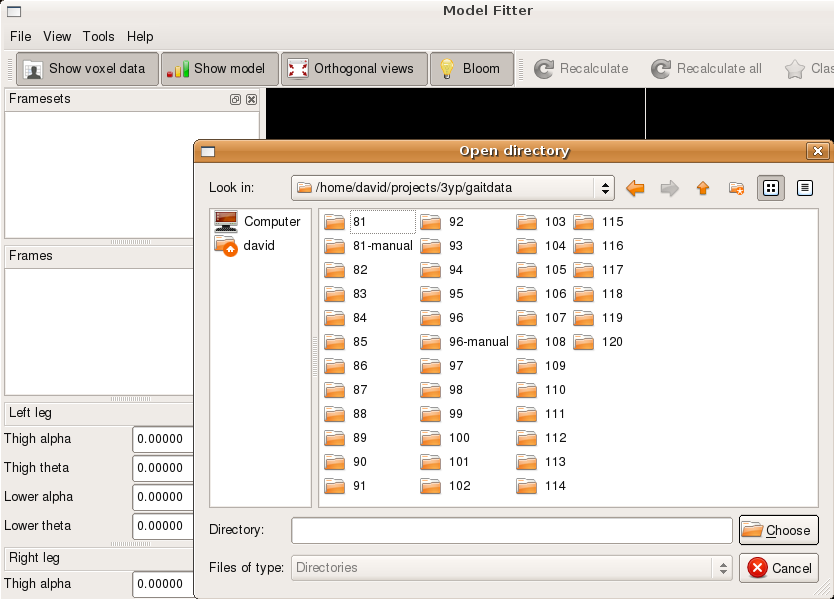
\includegraphics[width=8cm]{manual/opendir.png}
	\caption{Opening a directory containing gait samples.}
	\label{manual:opendir}
\end{figure}

The top-left, top-right and bottom-left views show front, side and overhead orthographic projections of the figure.
The bottom-right view shows a perspective projection.
This final view can be moved and rotated by the user with the following controls:

\begin{itemize}
	\item \textbf{Rotate} - click and drag inside the viewport.
	\item \textbf{Move} - hold the \emph{Shift} key, and click and drag inside the viewport.
\end{itemize}

The three orthographic projections can be toggled on and off by pressing the \emph{Orthogonal views} toolbar button.


\subsection{Model fitting and graph plotting}

Once you have selected a frame in the left dock panel you can start the modelfitting process by clicking the \emph{Recalculate} button on the toolbar.
This will open a progress dialog similar to the one shown in Figure \ref{manual:modelfitting}.

\begin{figure}[htb]
	\centering
	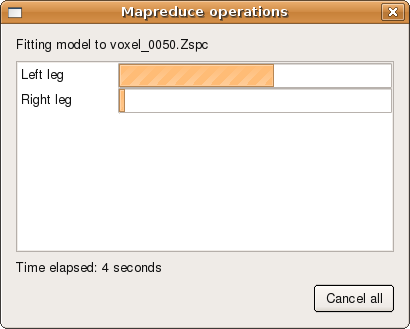
\includegraphics[width=6cm]{manual/modelfitting.png}
	\caption{Dialog displaying the progress of modelfitting operations.}
	\label{manual:modelfitting}
\end{figure}

The \emph{Recalculate All} button will run the modelfitting process on all the frames in the currently selected frameset.
Note that you can also process frames in bulk using the command line interface.
This is described in more detail in Section \ref{manual:commandline}

\bigskip
\noindent Several graph plotting facilities are available in the \emph{Tools} menu.
These all require the gnuplot utility to be installed and available in the system \$PATH.

\begin{itemize}
	\item \textbf{Plot energy graphs}.
		Only available immediately after the modelfitting process has completed.
		The data that is plotted is held in memory and not saved to disk, so it is discarded when opening another frame.
	\item \textbf{Plot params over time}.
		Plots the changes in the values of the various parameters over each of the frames in the frameset.
		Only frames that have previously had their model information calculated will be displayed in the graph.
		Figure \ref{manual:plotter} shows the graph plotting dialog.
	\item \textbf{Plot FFT graphs}.
		Runs a DFT on the data and displays the results.
		Magnitude and phase can be plotted individually, as well as the phase-weighted magnitude.
\end{itemize}

\begin{figure}[htb]
	\centering
	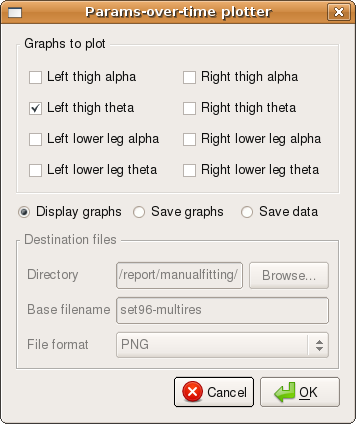
\includegraphics[width=6cm]{manual/plotter.png}
	\caption{A typical graph plotter dialog.}
	\label{manual:plotter}
\end{figure}

All graph dialogs have the option to display the graph, save the graph, or save the data that would be used to generate the graph.
The final option can be helpful if you need to use gnuplot manually to plot the data in different ways.


\subsection{Classification}

When you have calculated the model fitting for all frames in a frameset, you can click the \emph{Classify this Person} toolbar button to open the classification dialog.
When classifying a sample for the first time, the dialog will enter its signature into a database and use display it in a list for future classifications.
It will also display the ``distance'' from the sample you are classifying to all the other samples in the database.
This is a metric that determines the similarity between samples.

In Figure \ref{manual:classify} we can see that the sample being classified has a very similar gait to Sample 1 who was classified earlier.

\begin{figure}[htb]
	\centering
	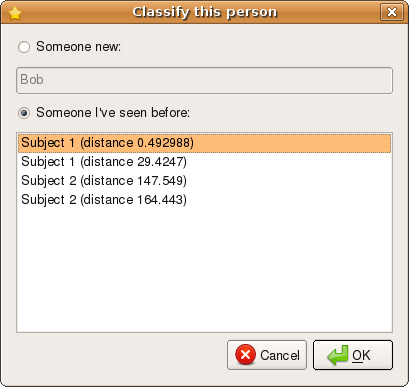
\includegraphics[width=6cm]{manual/classify.png}
	\caption{The classification dialog.}
	\label{manual:classify}
\end{figure}

Note that currently it is not possible to remove classifications from the database.
To do this you must edit the configuration directly:

\begin{itemize}
	\item \verb+~/.config/ECS/Modelfitting.conf+ on Unix
	\item \verb+~/Library/Preferences/uk.ac.soton.ecs.Modelfitting.plist+ on Mac OS X
	\item \verb+HKEY_CURRENT_USER\Software\ECS\Modelfitting+ on Windows
\end{itemize}


\clearpage
\section{Command line interface}
\label{manual:commandline}

It is possible to use the commandline interface to perform batch processing of frames on headless servers.

Note that sadly due to a bug in Qt it is not possible to use the command line interface on Unix without first applying a patch to the Qt sources.
The patch is provided on the DVD.
An issue has been raised with Trolltech and can be tracked by issue number 207245:

\verb+http://trolltech.com/developer/task-tracker+

\bigskip
\noindent A list of directories can be provided as commandline arguments to the modelfitting executable.
These will be processed sequentially:

\begin{lstlisting}[firstnumber=1,language=sh,frame=single]
$ ./modelfitting ../../gaitdata/81
Queueing all files in directory: ../../gaitdata/81
../../gaitdata/81/voxel_0058.Zspc: Starting...
../../gaitdata/81/voxel_0058.Zspc: Left leg finished

...
\end{lstlisting}

By default the thread pool creates one thread for every processor core in the system.
If one leg finishes processing before the other, one of these threads will sit idle and wait for the other leg to complete.
You can use the -j argument to specify the number of frames to process concurrently.
It is recommended to set this to 2 so that all the cores in the system will be working at any time.

\begin{lstlisting}[firstnumber=1,language=sh,frame=single]
$ ./modelfitting ../../gaitdata/81 -j 2
Queueing all files in directory: ../../gaitdata/81
../../gaitdata/81/voxel_0058.Zspc: Starting...
../../gaitdata/81/voxel_0059.Zspc: Starting...

...
\end{lstlisting}


\chapter{Developer documentation}
\section{Pre-requisites and compilation}

The complete source code for the application is included on the DVD.
It is also available from the subversion repository at:

\texttt{http://svn.davidsansome.com/3yp}

\bigskip
\noindent Before compiling you should make sure you have the following libraries and tools installed:

\begin{enumerate}
	\item \textbf{CMake} (\texttt{http://www.cmake.org}).
	\item \textbf{Qt} (\texttt{http://www.trolltech.com}).
		Version 4.4 is \emph{required} as the modelfitter application uses the new QtConcurrent framework.
		At the time of writing Qt 4.4 was in release-candidate stage.
	\item \textbf{SVL} (\verb+http://www.cs.cmu.edu/~ajw/doc/svl.html+).
		I have created an Ubuntu package for SVL which is available from: \\
		\texttt{http://www.davidsansome.com/svl}.
	\item \textbf{ZLib} (\texttt{http://www.zlib.net/}).
	\item \textbf{FFTW} (\texttt{http://www.fftw.org/}).
	\item \textbf{GnuPlot} (\texttt{http://www.gnuplot.info/}).
		Optional - but the GnuPlot executable should be installed and in the \$PATH at runtime if you want to use the application's graph plotting features.
\end{enumerate}

The application should compile cleanly on Linux, Mac OS X and Windows.
Windows users are advised to use MinGW instead of Visual Studio.
To build the application you should issue the following commands:

\begin{lstlisting}[firstnumber=1,language=sh,frame=single,morekeywords={cmake,make}]
cd modelfitting/bin
cmake ..
make
./modelfitting
\end{lstlisting}

\section{Code structure}
UML

\chapter{Code Listings}
\section{ThighFilter.m}
\lstset{language=Matlab}
\lstinputlisting[label=ThighFilter.m]{"../oldsource/ThighFilter.m"}

\newpage
\section{correlation.cg}
\lstset{language=Cg}
\lstinputlisting[label=correlation.cg]{"../oldsource/convolution.cg"}

\end{document}
